\documentclass[11pt, oneside]{article}   	
\usepackage{geometry}
\usepackage{hyperref}                		
\geometry{letterpaper}                   		
%\geometry{landscape}                	
%\usepackage[parfill]{parskip}
\usepackage{graphicx}
\usepackage{amssymb}

%SetFonts

%SetFonts

\graphicspath{ {./imgs/} } 			

\title{Visualizing Missing Values}
\author{Tommaso Romano - 941796}
%\date{}

\begin{document}
\maketitle

\tableofcontents
\pagebreak
\section{Introduzione}

Il seguente progetto di Visualizzazione Scientifica si occupa di analizzare, modificare e visualizzare dati provenienti da misurazioni cliniche. Pertanto, per diverse ragioni i dataset utilizzati sono disordinati e spesso contengono molti valori mancanti o duplicati. Potrebbero esserci più ragioni per la mancanza di tali dati, ma principalmente il motivo della loro assenza può essere attribuito a:
\begin{itemize}
\item Dati non esistono.
\item Dati non registrati per errore umano.
\item Dati cancellati accidentalmente.
\item Dati non registrati per malfunzionamento.
\end{itemize}

Ci occuperemo quindi di individuarli e modificarli per rendere il dataset utilizzabile per una corretta visualizzazione.

\subsection{Pyspark}

La tecnologia per gestire dataset, sarà PySpark invece di Pandas: PySpark è un'interfaccia per Apache Spark in Python. Non solo consente di scrivere applicazioni Spark usando le API Python, ma fornisce anche la shell PySpark per analizzare interattivamente i dati in un ambiente distribuito. PySpark supporta la maggior parte delle funzionalità di Spark come Spark SQL, DataFrame, Streaming, MLlib (Machine Learning) e Spark Core.

La scelta di utilizzare PySpark nel progetto è dovuta alla necessita di elaborare grosse quantità di dati, velocemente. Considerando l'enorme quantità di dati a disposizione, in questo progetto utilizzeremo solo una parte delle osservazione a disposizione, concentrandoci quindi su alcune condizioni cliniche. 

Ecco come inizializzare PySpark e creare i DataFrame:
\begin{center}
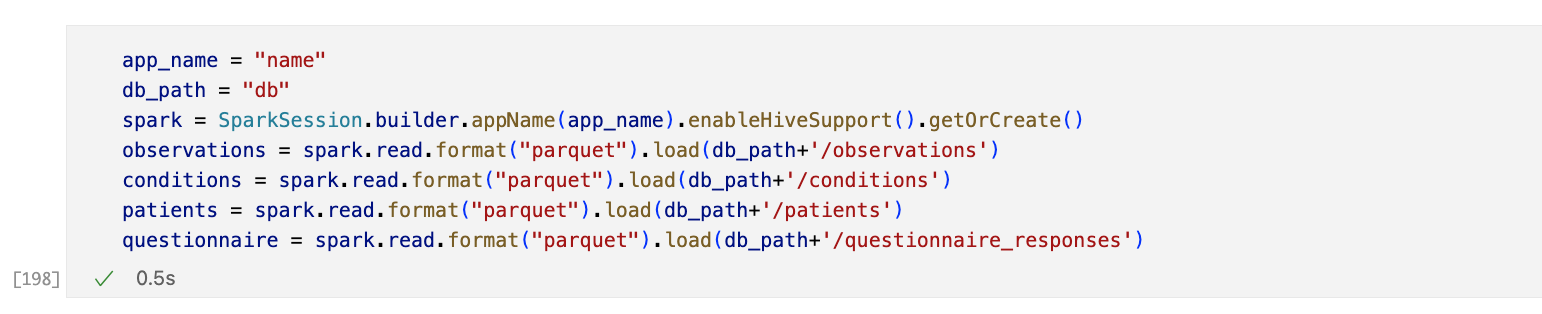
\includegraphics[scale=0.5]{1_init.png}
\end{center}

PySpark offre la possibilità di visualizzare il corrente DataFrame come stringa tramite il comando \emph{.show()}:

\begin{center}
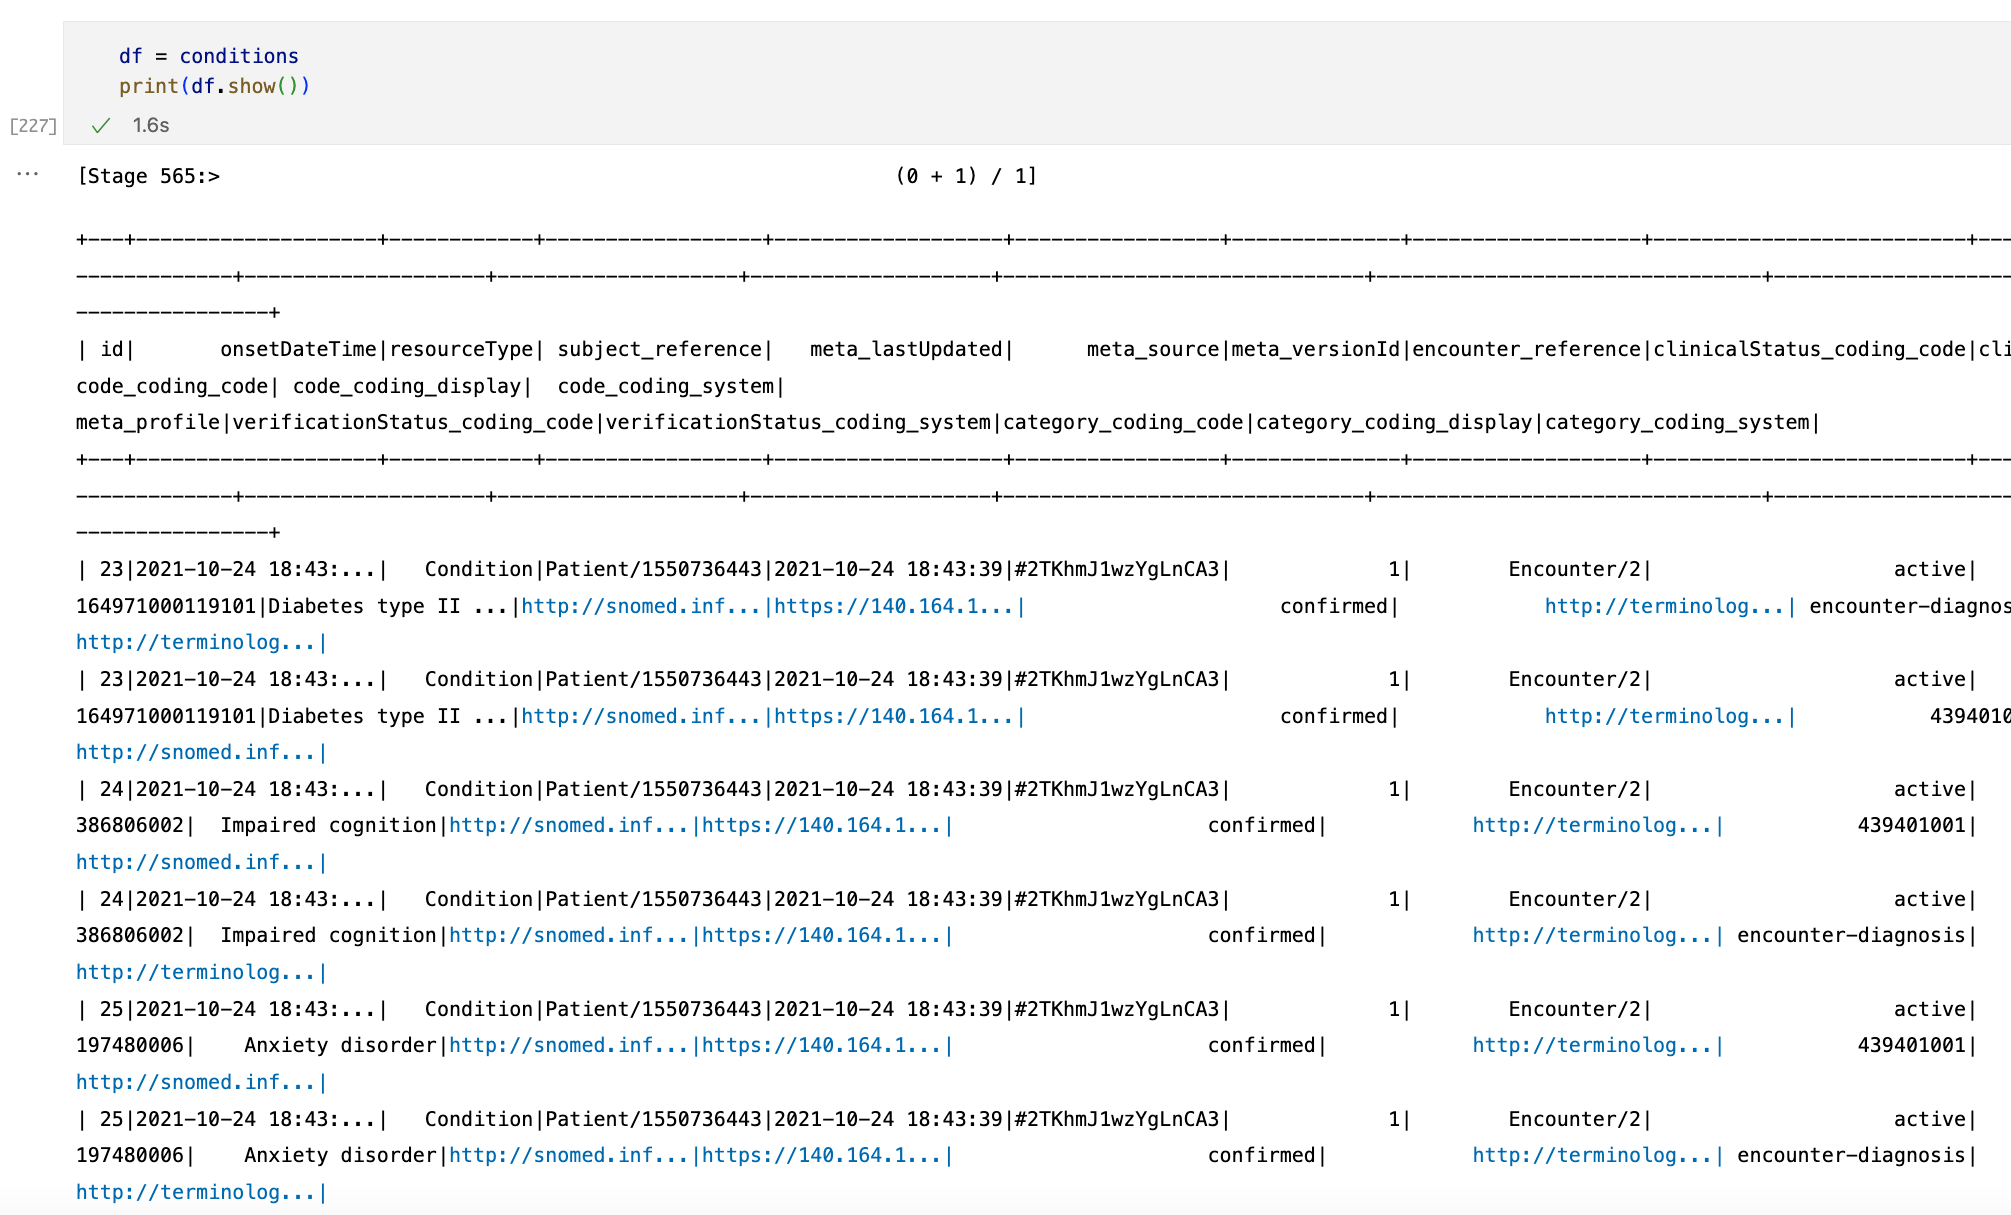
\includegraphics[scale=0.5]{1_spark.png}
\end{center}

Come si può vedere, la visualizzazione tramite stringa, viene distorta ed è a fatica comprensibile. Questo è dovuto alla grande quantità di colonne e l'utilizzo di Jupyter Notebook. Pertanto, dato che ridurremo il numero delle osservazioni, trasformeremo il DataFrame di PySpark in Pandas per visualizzare meglio i risultati:

\begin{center}
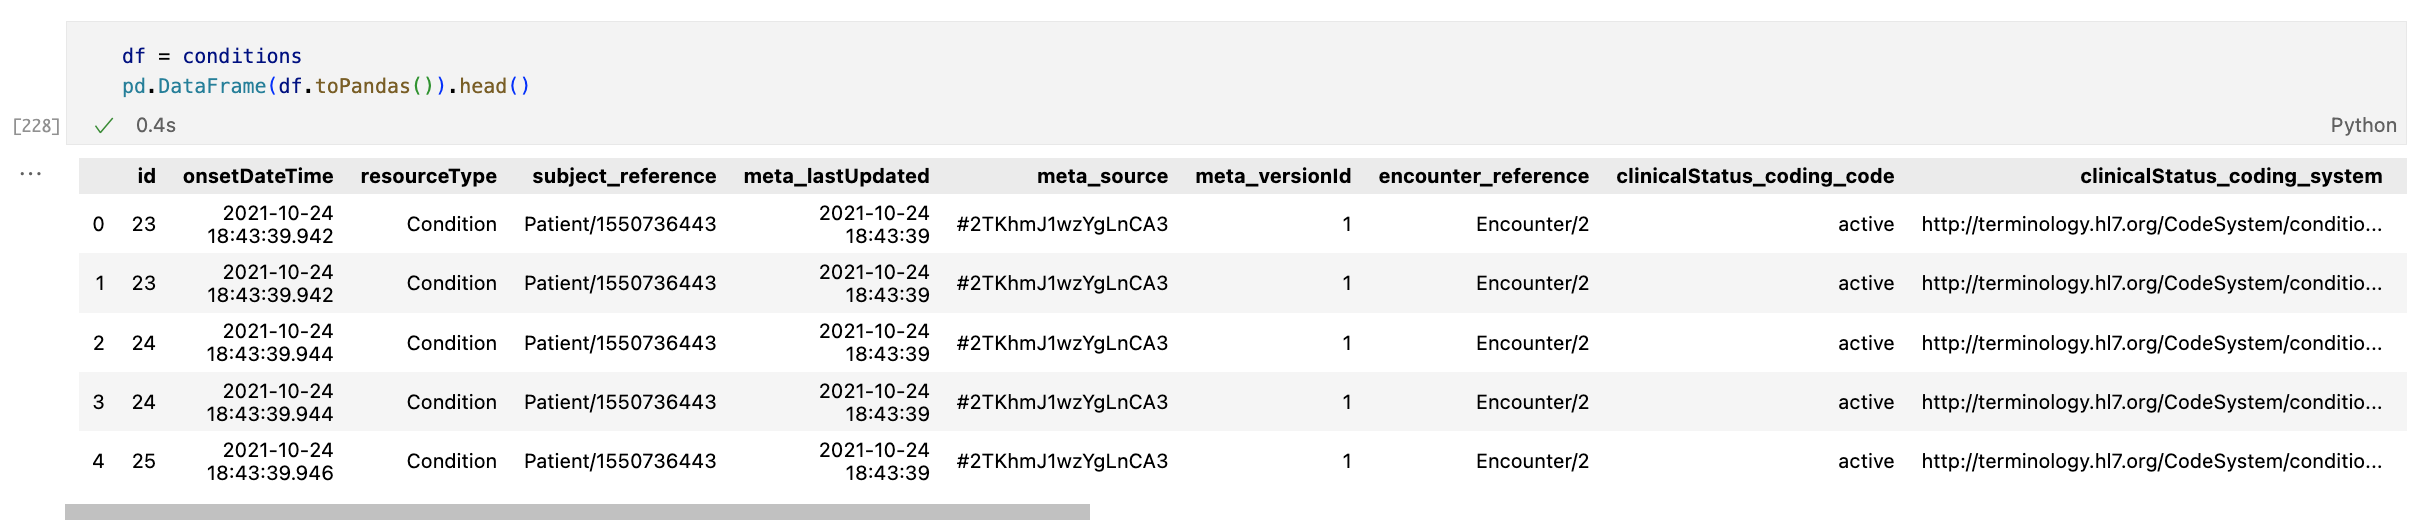
\includegraphics[scale=0.5]{1_pandas.png}
\end{center}


\subsection{ECharts}

Un'altra tecnologia che useremo in questo progetto è ECharts di Apache: è uno strumento di visualizzazione JavaScript open source, che può essere eseguito in modo fluido su PC e dispositivi mobili. Infatti, a differenza dei grafici statici di matplot, ECharts offre una soluzione dinamica ed interattiva, oltre che ad una gamma più ampia e maggiormente personalizzabile di grafici.


Echarts, per funzionare su Python ha bisogno di una libreria come \emph{pyecharts}. Una galleria dinamica di esempio ufficiale di Apache si trova al \href{https://echarts.apache.org/examples/en/index.html}{seguente link}, mentre delle gif di esempio di cui ho riportato sotto un fermo immagine, si trovano al \href{https://github.com/pyecharts/pyecharts#-demo}{seguente link}.

\begin{center}
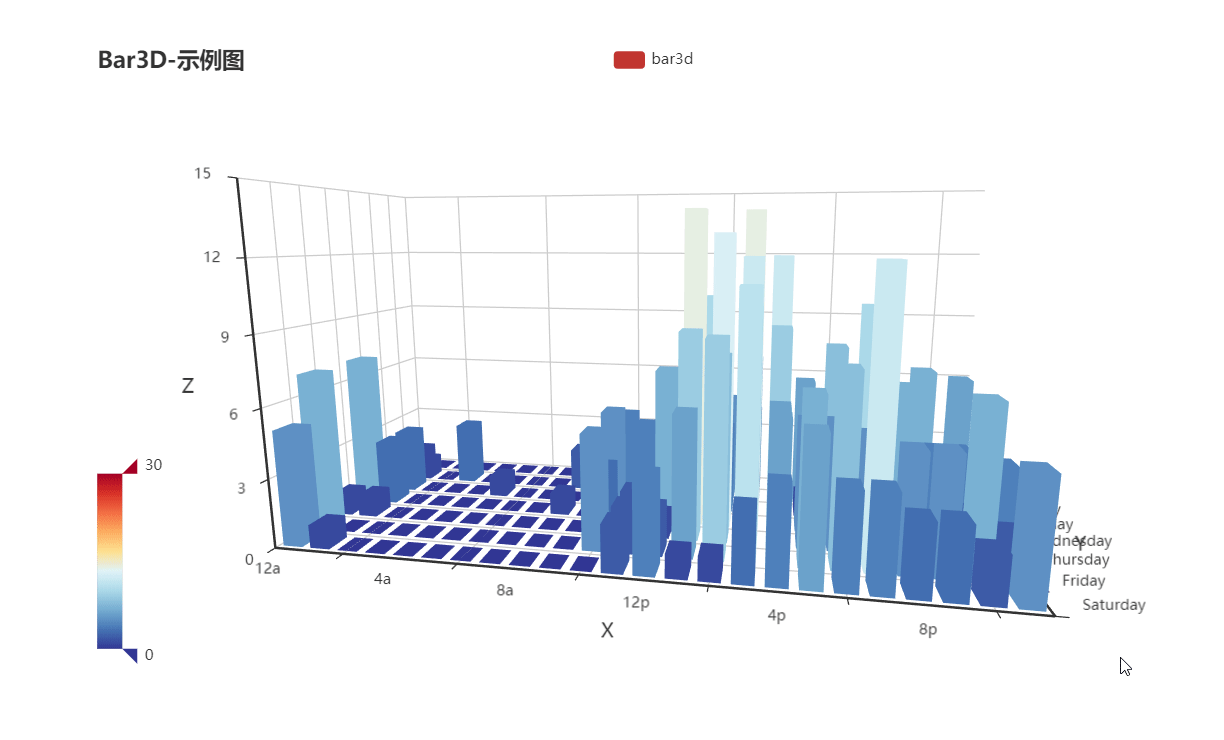
\includegraphics[scale=0.3]{1_echarts_1.png}
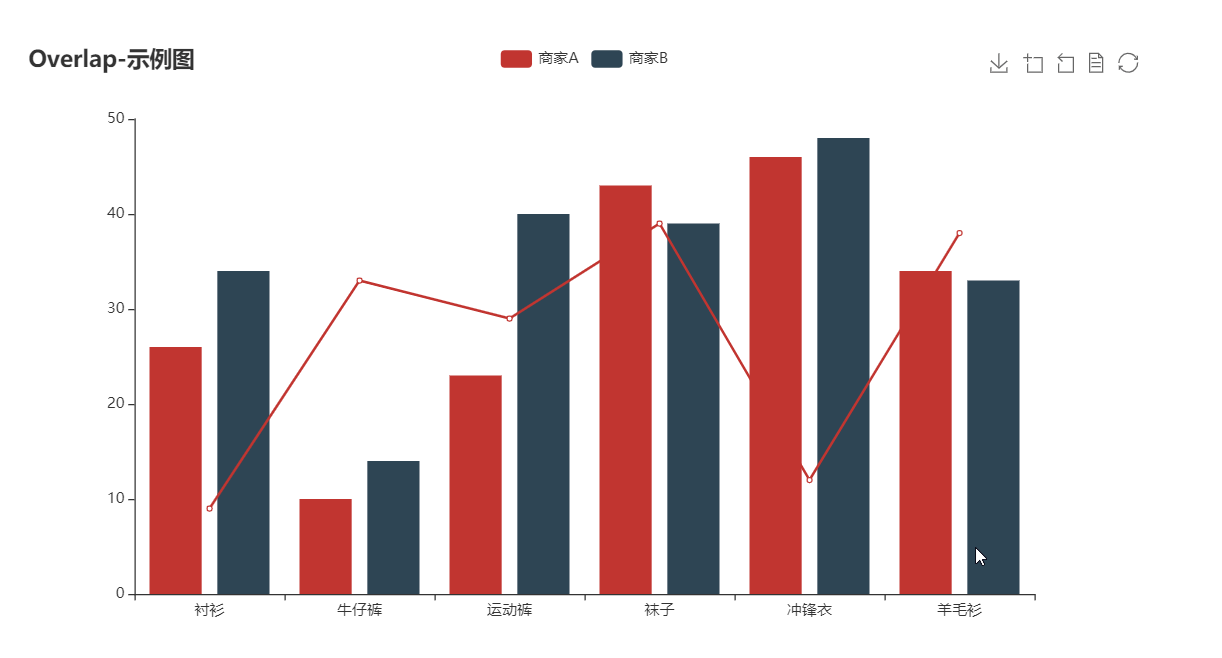
\includegraphics[scale=0.3]{1_echarts_2.png}
\end{center}

\subsection{Conditions}

Iniziamo utilizzando il dataset delle \emph{conditions} per identificare il numero di pazienti che sono seguiti per una data condizione clinica. Il DataFrame contiene 19 colonne che sono \emph{'id', 'onsetDateTime', 'resourceType', 'subject\_reference', 'meta\_lastUpdated', 'meta\_source', 'meta\_versionId', 'encounter\_reference', 'clinicalStatus\_coding\_code', 'clinicalStatus\_coding\_system', 'code\_coding\_code', 'code\_coding\_display', 'code\_coding\_system', 'meta\_profile', 'verificationStatus\_coding\_code', 'verificationStatus\_coding\_system', 'category\_coding\_code', 'category\_coding\_display','category\_coding\_system'} e ci serviranno solamente \emph{clinicalStatus\_coding\_code, code\_coding\_display} in modo tale da filtrare per pazienti marcati come \emph{active} e tramite PySpark, come per SQL raggrupparli tramite \emph{.groupBy()} per nome della condizione, conteggiarli ed ordinarli in modo discendente:

\begin{center}
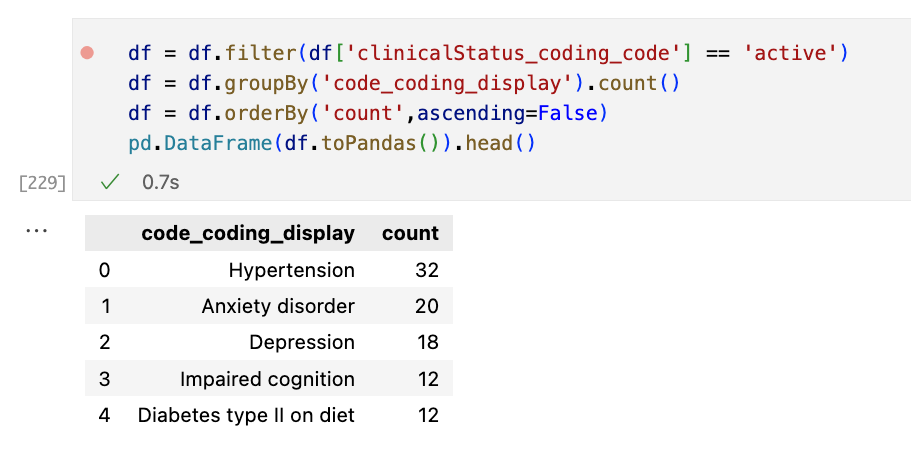
\includegraphics[scale=0.5]{1_conditions.png}
\end{center}

Il secondo step è visualizzare i dati raccolti. Sicuramente il modo più facile per organizzare i dati categorici raccolti è tramite un grafico a barre. Tramite ECharts creo il grafico dinamico che è possibile scaricare al \href{https://github.com/tommasoromano/scientific-vision/blob/main/renderers/bar_conditions.html}{seguente link}:

\begin{center}
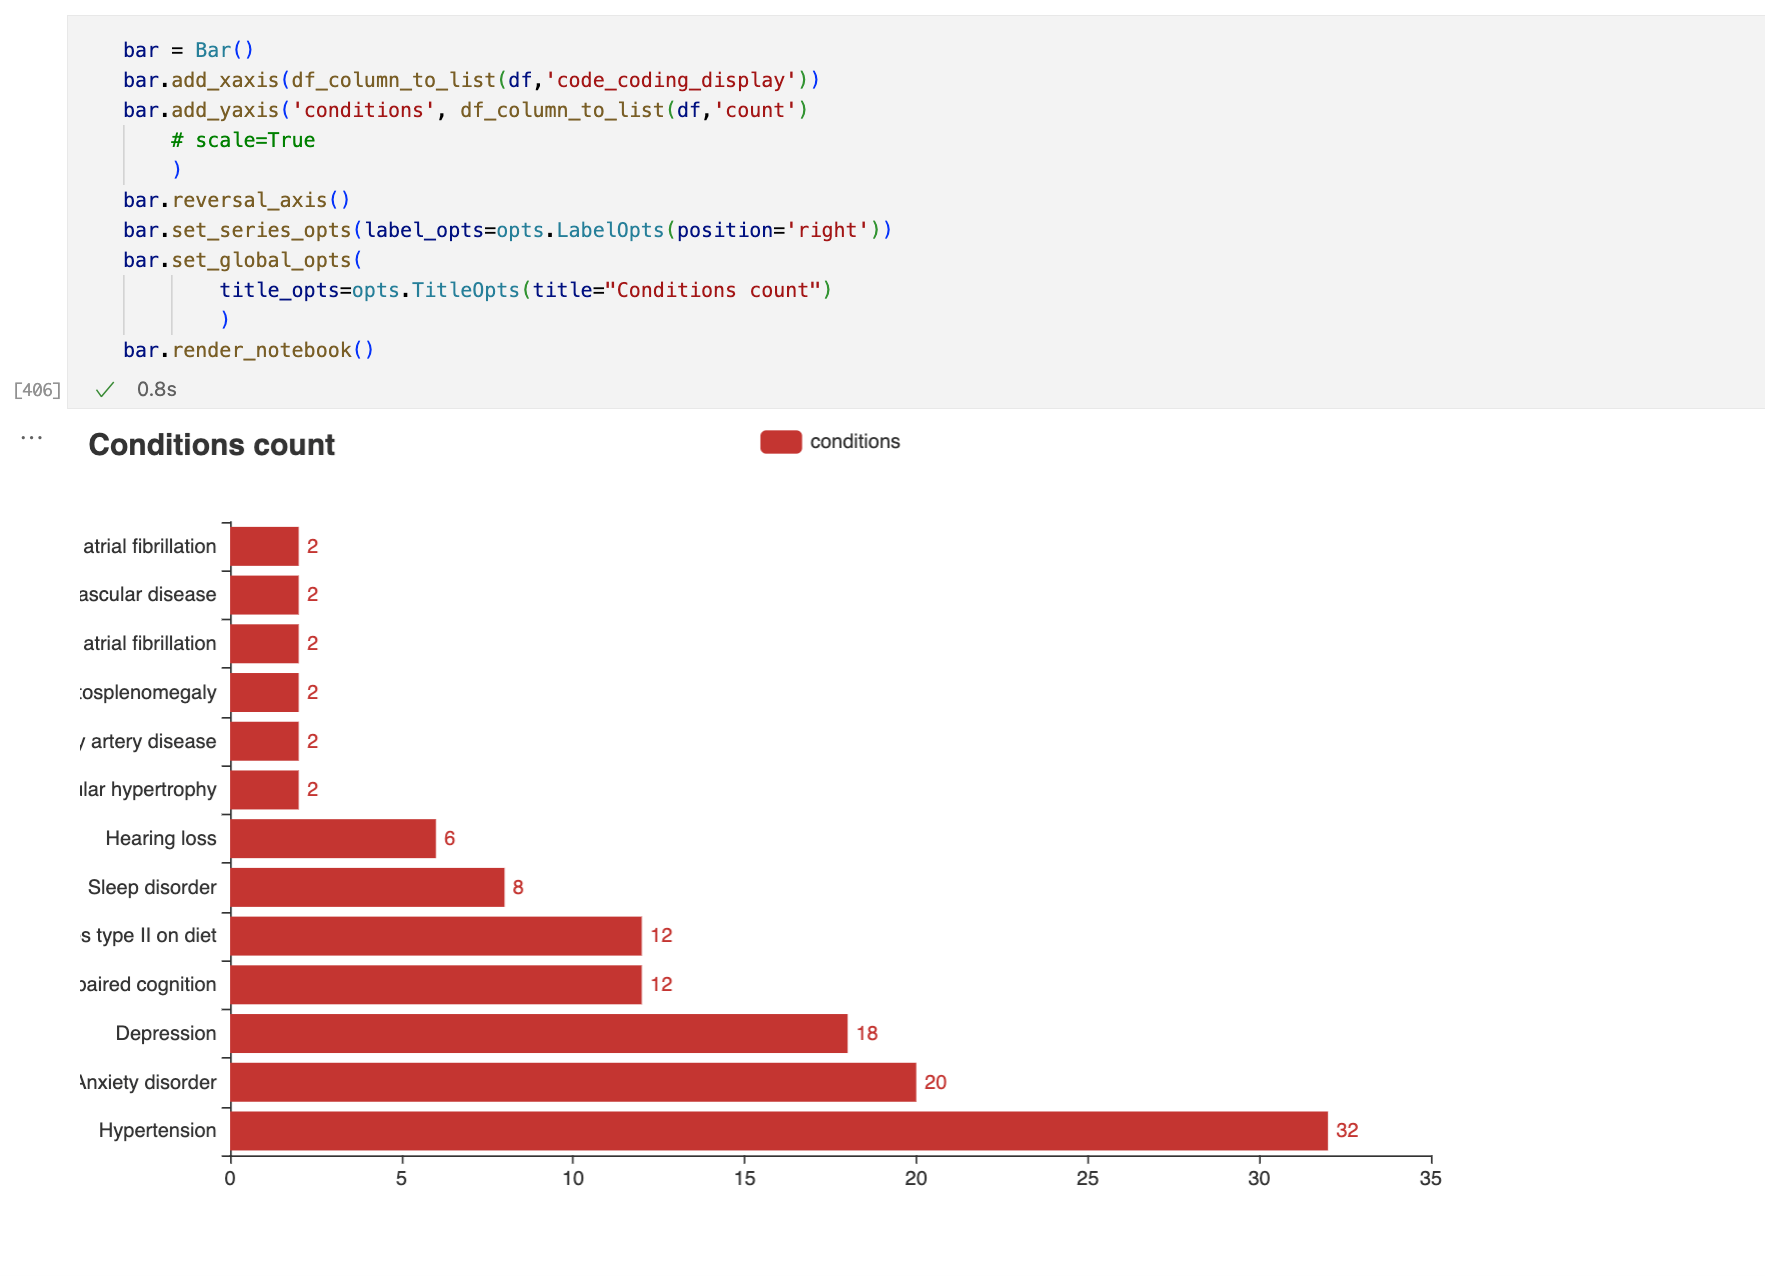
\includegraphics[scale=0.5]{1_bars.png}
\end{center}

Un altro modo per visualizzare e comparare i dati categorici, simile al grafico a barre ma più originale è il Funnel al \href{https://github.com/tommasoromano/scientific-vision/blob/main/renderers/funnel_conditions.html}{seguente link}:

\begin{center}
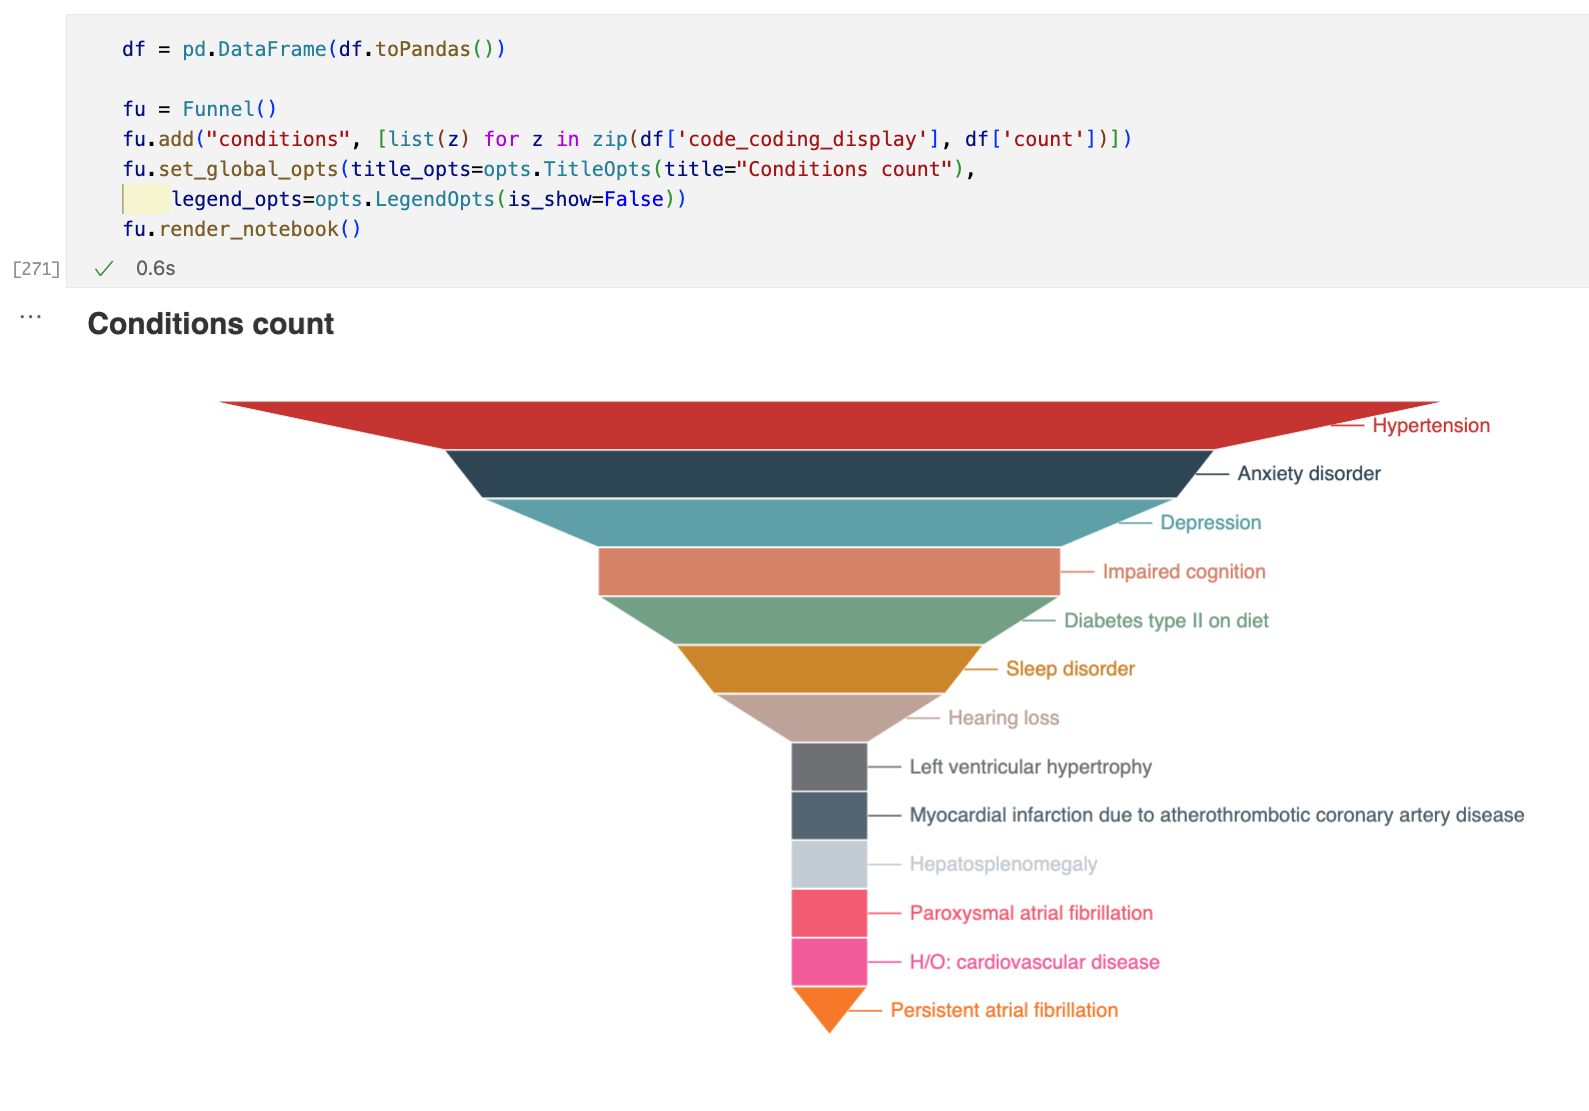
\includegraphics[scale=0.5]{1_funnel.png}
\end{center}

\section{Missing data}

Terminata la visualizzazione delle condizioni esistenti dei pazienti, ci occupiamo della visualizzazione delle osservazioni delle diverse condizioni cliniche. Il DatFrame che utilizzeremo contiene 63 colonne, ovvero: \emph{effectiveDateTime', 'id', 'resourceType', 'status', 'valueInteger', 'valueQuantity\_code', 'valueQuantity\_system', 'valueQuantity\_unit', 'valueQuantity\_value', 'subject\_reference', 'meta\_lastUpdated', 'meta\_source', 'meta\_versionId', 'encounter\_reference', 'bodySite\_coding\_code', 'bodySite\_coding\_display', 'bodySite\_coding\_system', 'code\_coding\_code', 'code\_coding\_display', 'code\_coding\_system', 'meta\_profile', 'valueCodeableConcept\_coding\_code', 'valueCodeableConcept\_coding\_display', 'valueCodeableConcept\_coding\_system', 'component\_valueQuantity\_code', 'component\_valueQuantity\_system', 'component\_valueQuantity\_unit', 'component\_valueQuantity\_value', 'component\_code\_coding\_code', 'component\_code\_coding\_display', 'component\_code\_coding\_system', 'valueBoolean', 'valueSampledData\_data', 'valueSampledData\_dimensions', 'valueSampledData\_lowerLimit', 'valueSampledData\_period', 'valueSampledData\_upperLimit', 'valueSampledData\_origin\_code', 'valueSampledData\_origin\_system', 'valueSampledData\_origin\_unit', 'valueSampledData\_origin\_value', 'effectivePeriod\_end', 'effectivePeriod\_start', 'code\_text', 'category\_coding\_code', 'categor\_coding\_display', 'category\_coding\_system', 'identifier\_system', 'identifier\_value', 'extension\_url', 'extension\_valueCodeableConcept\_coding\_code', 'extension\_valueCodeableConcept\_coding\_display', 'extension\_valueCodeableConcept\_coding\_system', 'component\_valueSampledData\_data', 'component\_valueSampledData\_dimensions', 'component\_valueSampledData\_period', 'component\_valueSampledData\_origin\_code', 'component\_valueSampledData\_origin\_system', 'component\_valueSampledData\_origin\_unit', 'component\_code\_text', 'component\_code\_coding\_version', 'component\_valueSampledData\_extension\_url', 'component\_valueSampledData\_extension\_valueString'}.

\begin{center}
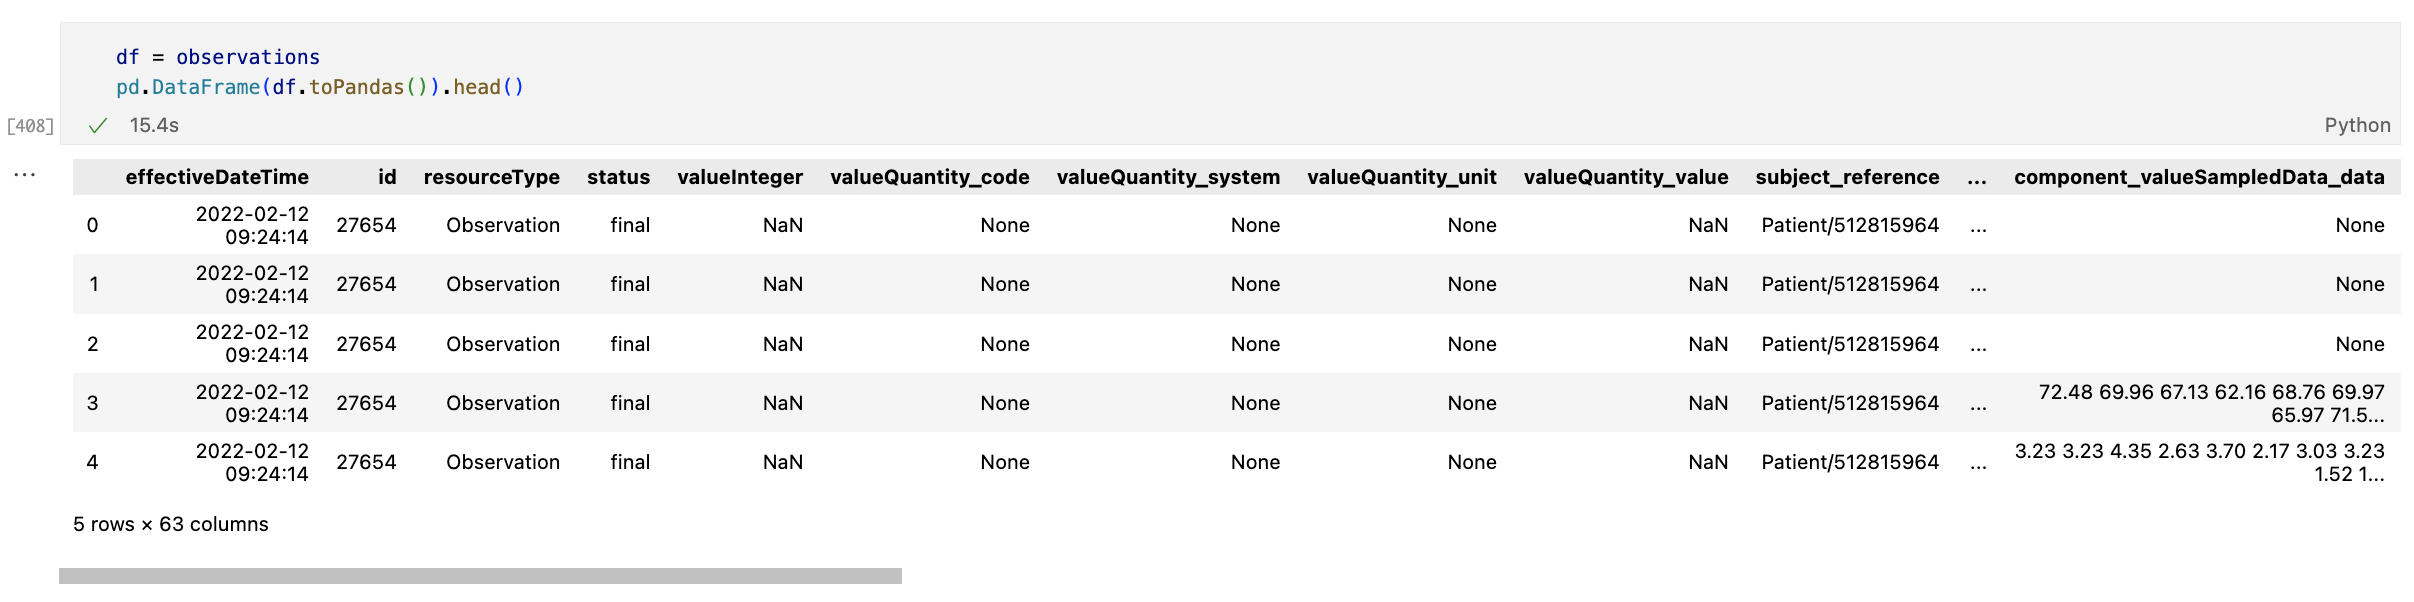
\includegraphics[scale=0.45]{2_obs.png}
\end{center}

Di questi 63 attributi, ne useremo solamente alcuni per determinati tipi di condizioni cliniche e pazienti. Infatti, molti di questi contengono molti se non tutti valori nulli o mancanti. Un metodo alternativo e visivo per identificare missing values è tramite l'utilizzo di grafici come quello a barre, delle matrici o heatmap.

\subsection{Missingno}

Una libreria utile a visualizzare i dati macanti è sicuramente \emph{Missigno}. Infatti, contiene tre grafici particolari (bars, matrix e heatmap) che consentono di visualizzare facilmente ed efficacemente DataFrame con la presenza di dati mancanti, e comprendere i motivi per cui i dati non sono presenti.

\begin{center}
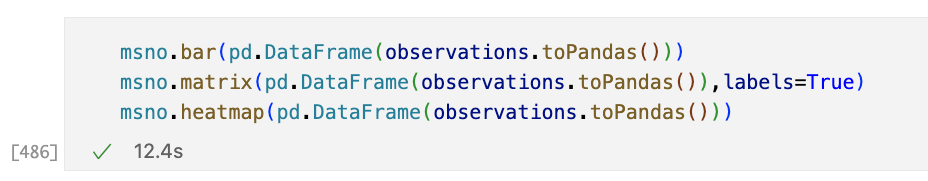
\includegraphics[scale=0.45]{2_msn.png}
\end{center}

Il più facile grafico è sicuramente quello a barre che evidenzia per ogni attributo la quantità di dati presenti rispetto al totale delle osservazioni. Notare come nel DatFrame utilizzato, molti attributi contengano 0 valori e altri solamente una frazione delle osservazioni totali. 

\begin{center}
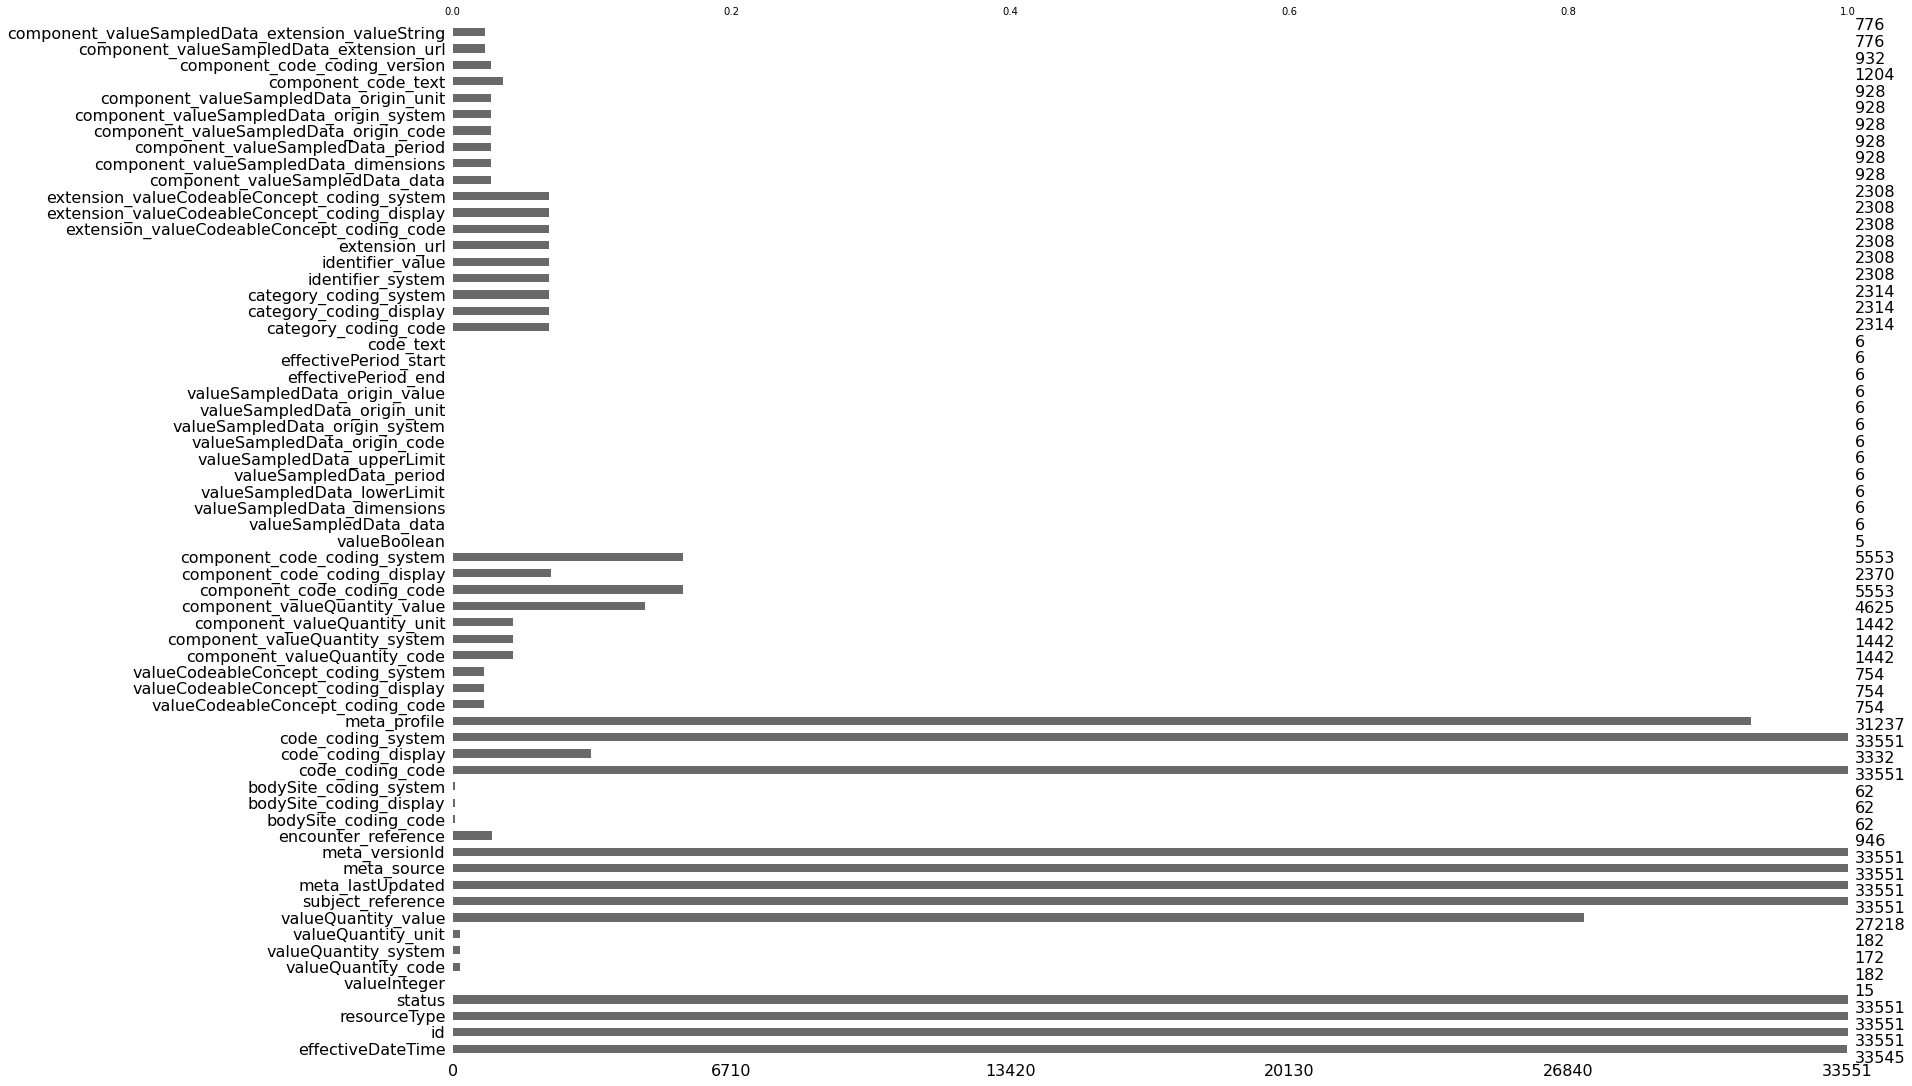
\includegraphics[scale=0.2]{2_msn_bars.png}
\end{center}

La matrice qui sotto invece, aggiunge informazioni molto importanti rispetto al grafico precedente: permette di analizzare visivamente dove (ovvero in quale riga del DataFrame) i dati sono mancanti. Infatti, presenta un ulteriore strumento alla sua destra che è il \emph{Data Completeness} che descrive in una data riga quanti sono i dati presenti rispetto a quelli mancanti. 

\begin{center}
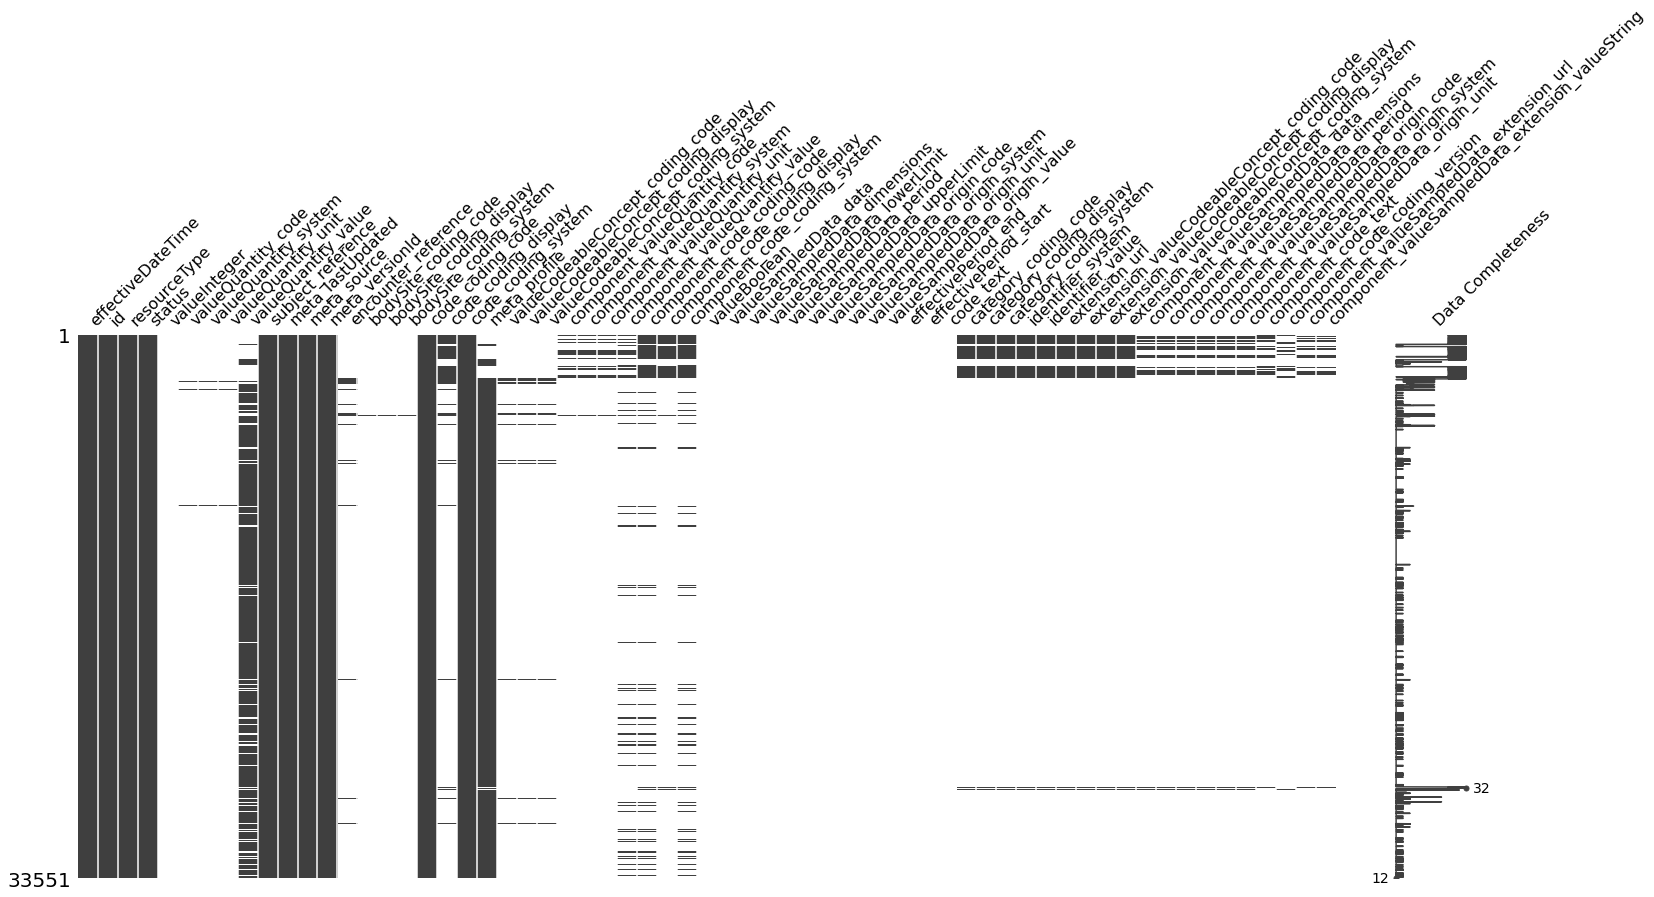
\includegraphics[scale=0.25]{2_msn_matrix.png}
\end{center}

Infine la Heatmap permette di visualizzare un altro elemento importante: la correlazione tra i diversi dati. In particolare, consente di identificare motivi di missing values relativi alla relazione tra due attributi.

\begin{center}
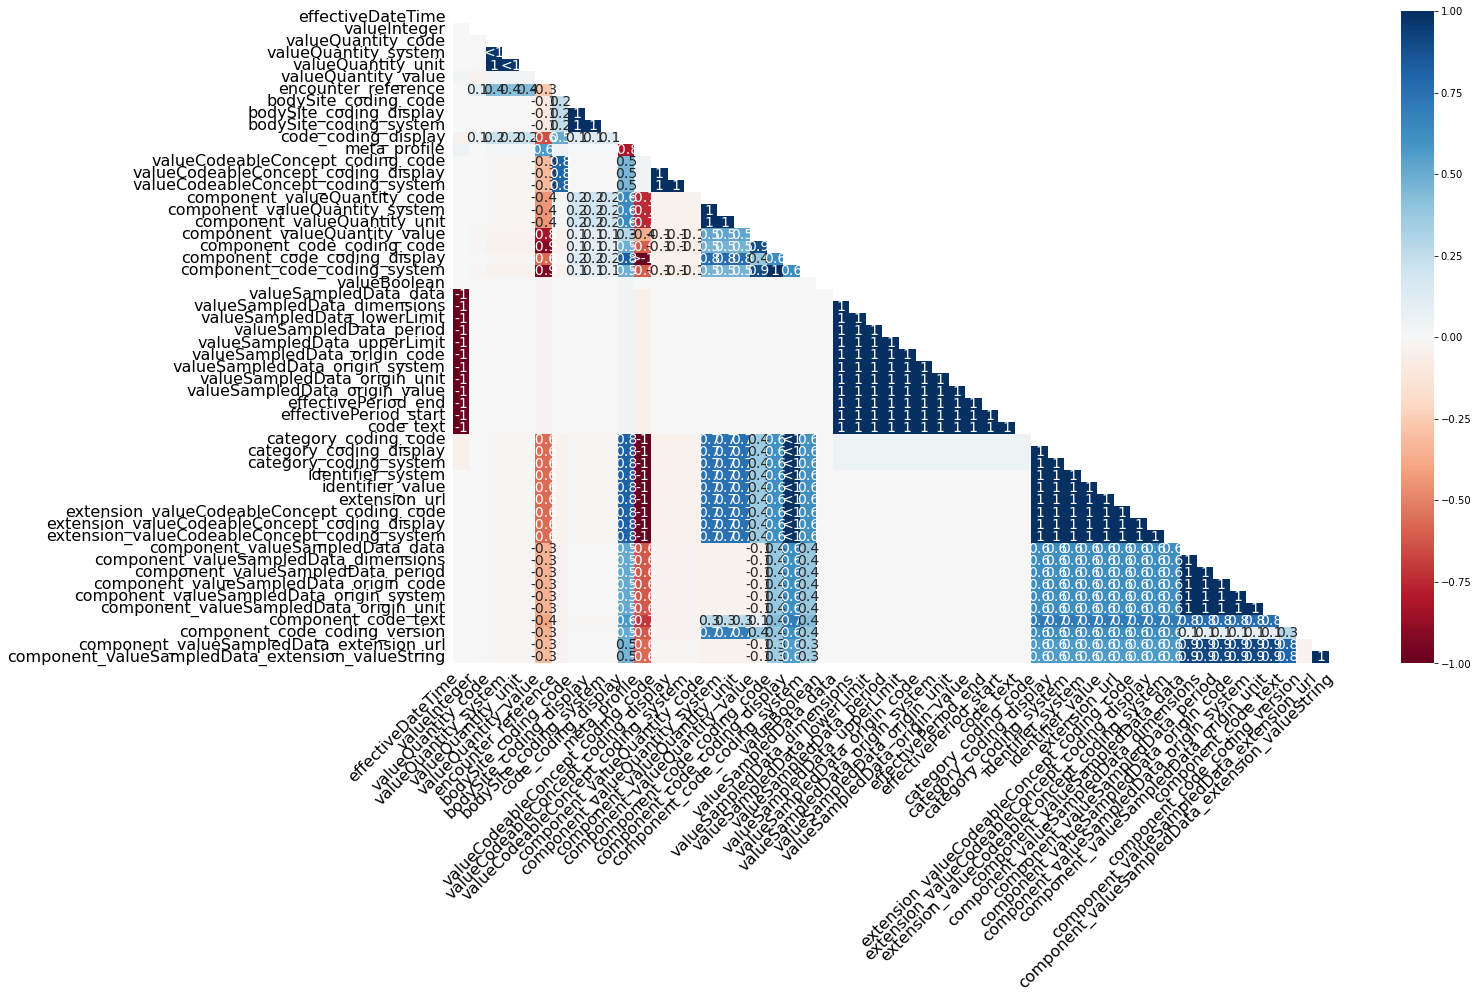
\includegraphics[scale=0.25]{2_msn_heatmap.png}
\end{center}

A causa dell'elevato numero di attributi nel DataFrame, nei grafici precedenti, la visualizzazione risulta perlopiù confusionaria. Occorre quindi ridurre il numero di colonne, eliminando ad esempio quelle che contengono zero valori, oppure quelle che ne contengono sotto una percentuale fornita dall'utente. Successivamente a questa modifica, i grafici saranno sicuramente più di facile comprensione.

\subsection{Filter}

Per filtrare le osservazione e ridurre il numero di colonne, si può procedere eliminando ad esempio quelle contenenti zero osservazioni o eliminando quelle che contengono un numero di osservazioni sotto una certa soglia. Infatti molti attributi del dataset che stiamo utilizzando, sono stati inseriti per osservazioni future o per misurazioni non più di alcun utilizzo.

Pertanto, per l'analisi di dati che svilupperemo successivamente, utilizzeremo solamente 6: \emph{subject\_reference, effectiveDateTime, code\_coding\_code, component\_code\_coding\_code, valueQuantity\_value, component\_valueQuantity\_value}. Questi attributi corrispondono rispettivamente a: id del paziente esaminato, il timestamp della registrazione della misurazione, il codice genitore dell'osservazione, il codice foglio dell'osservazione, il valore legato al codice padre dell'osservazione, il valore legato al codice figlio della misurazione.

Per filtrare efficacemente le osservazioni, creiamo queste due funzioni:

\begin{center}
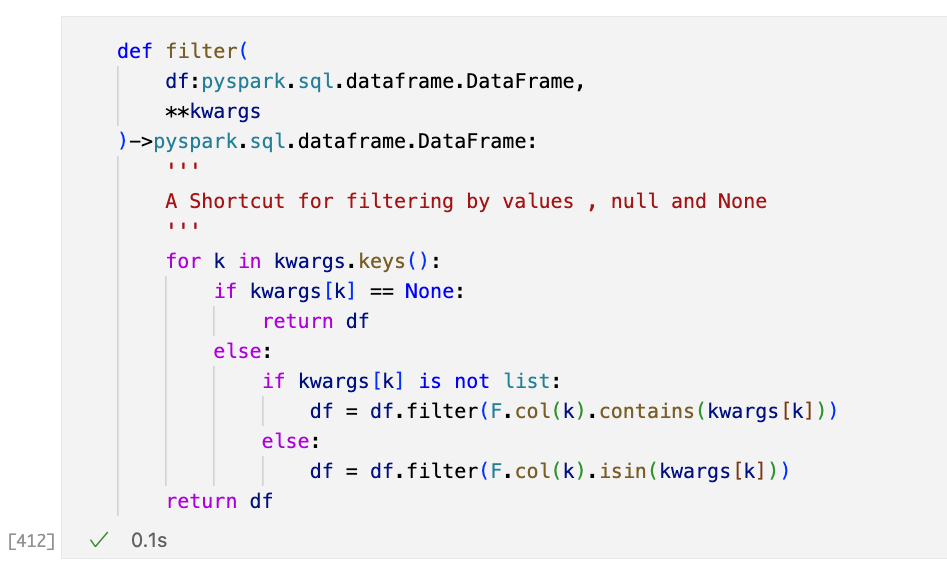
\includegraphics[scale=0.45]{2_filter.png}
\end{center}

La funzione atomica/generale \emph{filter ( df, **kwargs )} permette di filtrare da un qualsiasi DataFrame PySpark in base ad una qualsiasi colonna ed un valore o una lista di valori.

\begin{center}
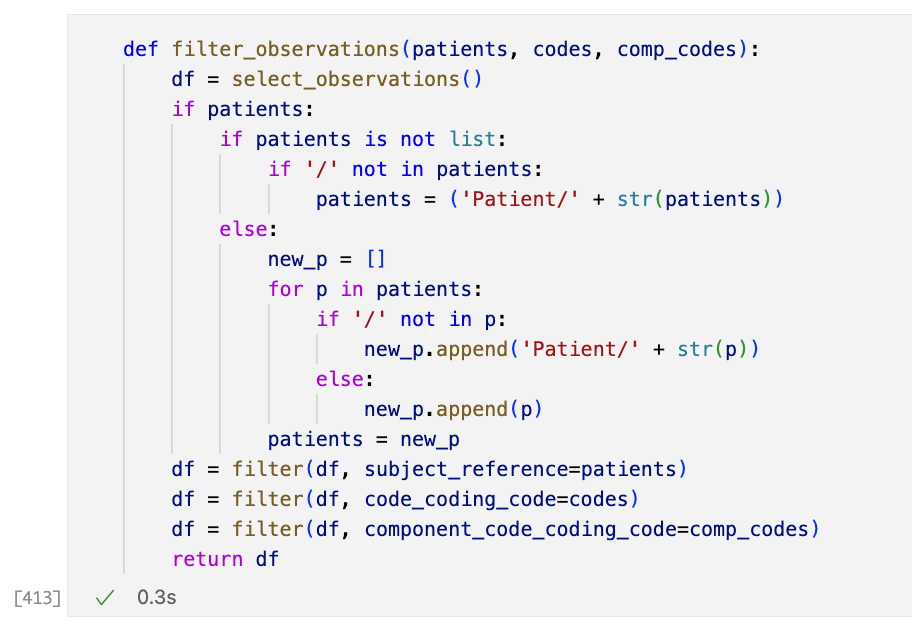
\includegraphics[scale=0.45]{2_filter_obs.png}
\end{center}

La funzioni \emph{filter\_observations ( patients, codes, comp\_codes )} è invece specifica per questo dataset per velocizzare molti pattern, ed utilizza la funzione atomica/generale filter insieme ad una di select delle colonne utili per le osservazioni che useremo.

\begin{center}
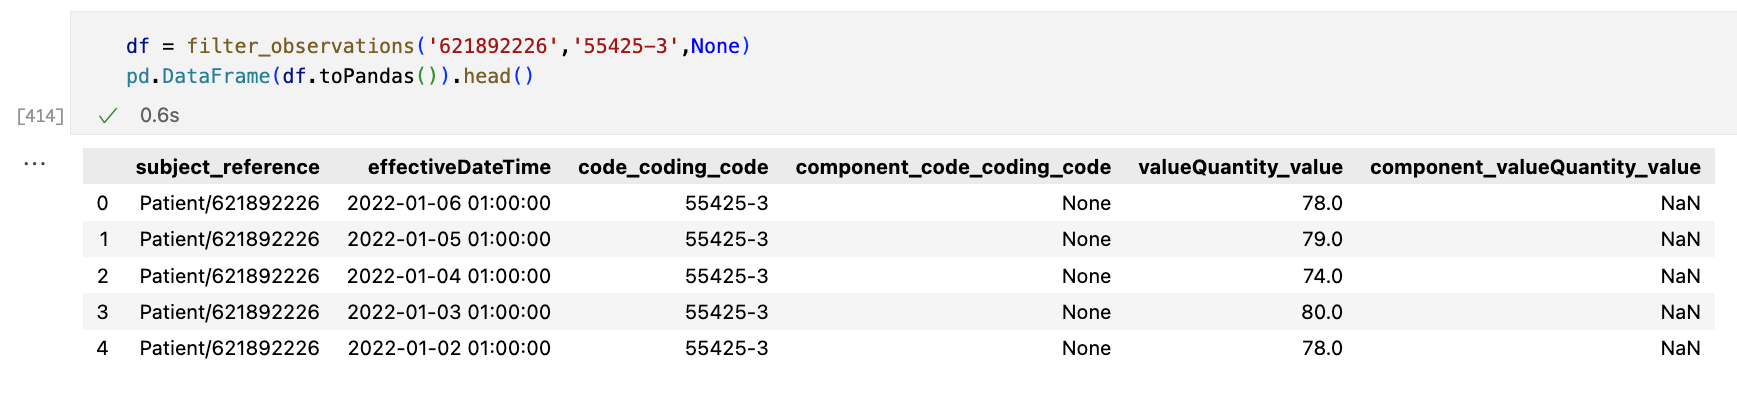
\includegraphics[scale=0.45]{2_filter_obs_df.png}
\end{center}

Grazie a queste funzioni possiamo ora visualizzare più efficacemente il grafico matrix per determinare la presenza o assenza di missing values per il paziente \emph{621892226} e condizione \emph{55425-3} (ovvero Heart Beats) che saranno i nostri dati di riferimento per le prossime osservazioni. 

\begin{center}
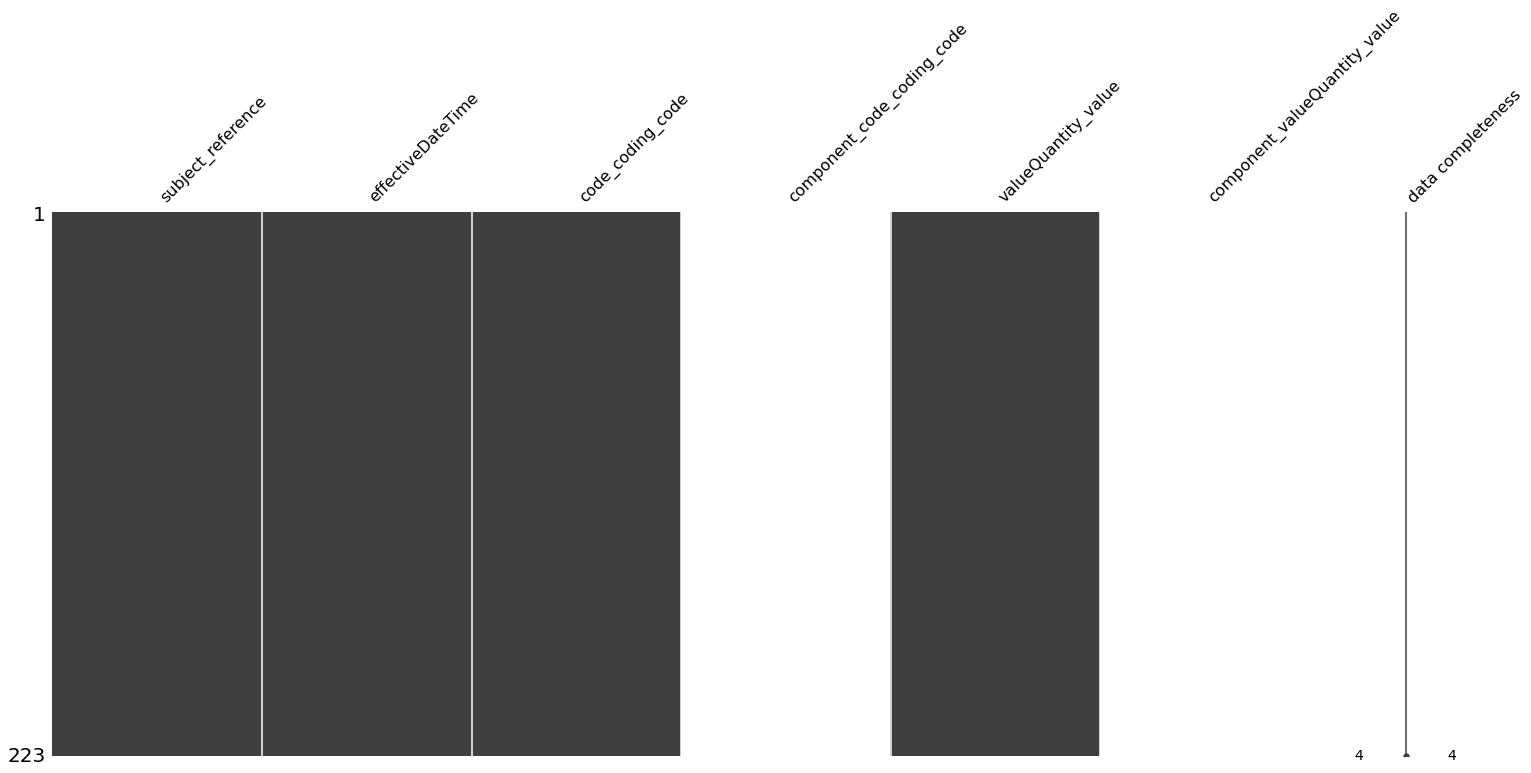
\includegraphics[scale=0.25]{2_msn_df.png}
\end{center}

Come si può vedere dal grafico, i dati sono completi e non sono presenti dati mancanti. Infatti, i dati legati agli attributi component* non sono necessari per le osservazioni di Heart Beats. Ma siamo sicuri che non ci siano dati mancanti?

\section{Imputation}

Nelle precedenti analisi del DataFrame per identificare i missing values ci siamo occupati di setacciare solamente la relazione tra il codice della condizione con il codice di un paziente per trovare i valori. Tuttavia se volessimo creare un grafico che visualizza la media del battito cardiaco di giorno in giorno, potremmo ritrovare un'altra categoria di missing values che sono legati alla time sieries

\subsection{Time Series}

Utilizziamo il DataFrame creato nei punti precedenti ed ordiniamolo secondo il timestamp della rilevazione. Ci possiamo facilmente accorgere che tra il 2021-11-15 e 2021-12-10 non ci sono state rilevazioni del battito cardiaco. Questo perchè, quando ci si occupa di rilevazioni che non sono fatte automaticamente da un software, ma affidandosi unicamente alla rilevazione di un utente, si possono trovare numerosi dati mancanti o duplicati in un dato arco temporale oppure più rilevazioni in brevi periodi.

\begin{center}
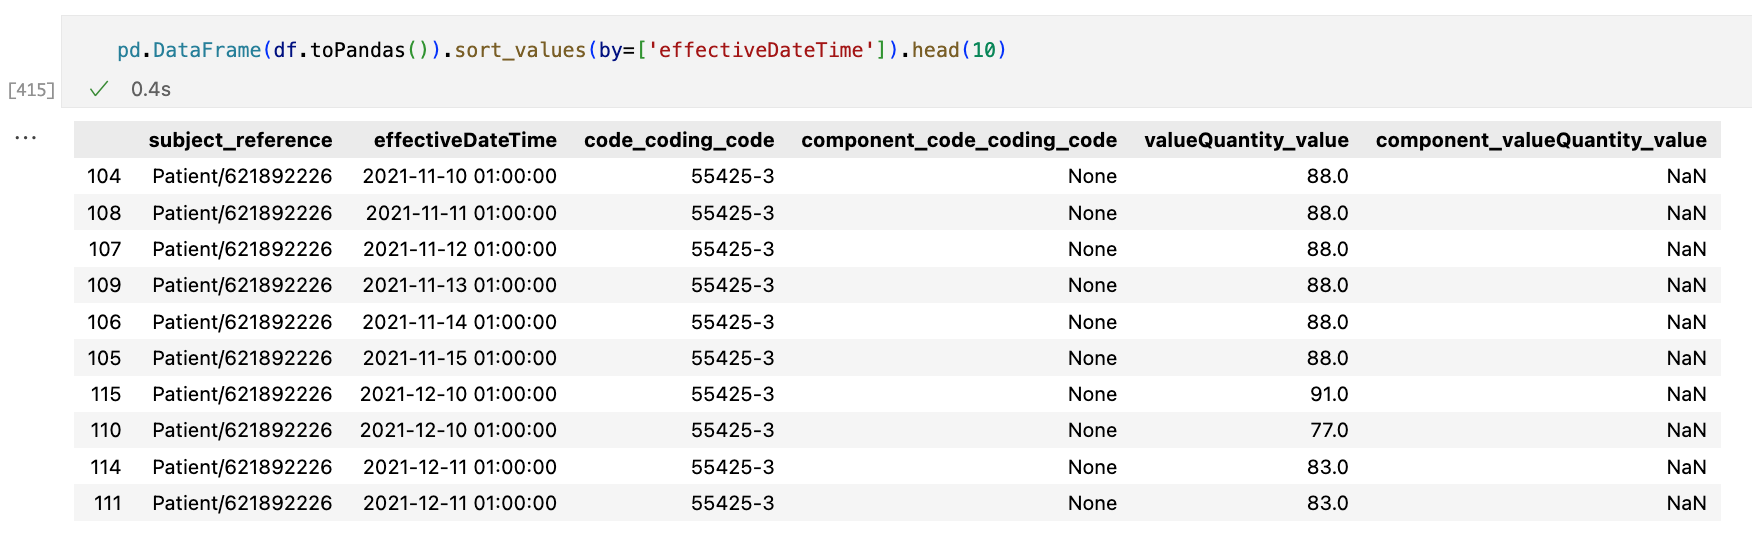
\includegraphics[scale=0.45]{2_sort.png}
\end{center}

Nel DataFrame precedente sono inoltre presenti più rilevazioni al giorno (ad esempio 2021-12-11) e se volessimo visualizzare un grafico giorno per giorno ci troveremmo giorni duplicati. Occorre quindi creare un funzione che raggruppa i dati temporali per una quantità che possiamo definire noi (come ad esempio ore, giorni, settimane o mesi). Utilizziamo una funzione già esistente di PySpark (\emph{date\_trunc}) e successivamente raggruppiamo per l'intervallo di tempo selezionato con quelle colonne che sono immutabili alle osservazioni. Infine processiamo i gruppi creati con una funzione semplice come la media.

\begin{center}
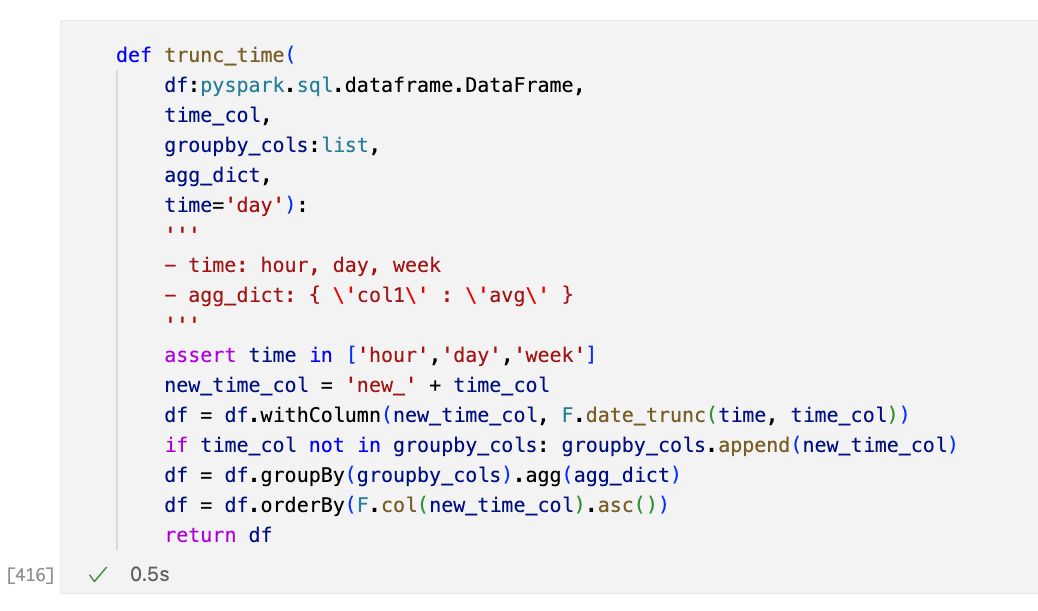
\includegraphics[scale=0.45]{3_trunc.png}
\end{center}

\begin{center}
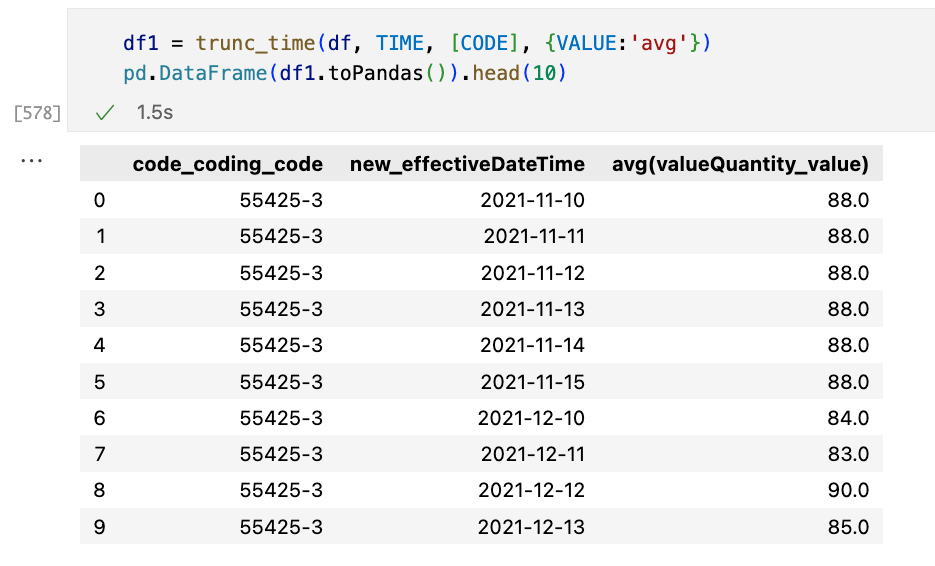
\includegraphics[scale=0.45]{3_trunc_df.png}
\end{center}

Il DataFrame ottenuto non contiene intervalli di tempi duplicati per ora, giorno, settimana o mese. Tuttavia, non è ancora risolta la presenza di timestamp mancanti come quelli tra 2021-11-15 e 2021-12-10. Creiamo quindi la funzione \emph{fill\_missing\_time\_values ( df, ... )} che in base all'intervallo di tempo selezionato aggiunge righe di dati vuoti inserendo i timestamp mancanti. Nel dataset precedente quindi inserirebbe le date dal 2021-11-14 al 2021-12-09 con None or NaN a seconda dei tipi di attributi diversi dalle time values.

\begin{center}
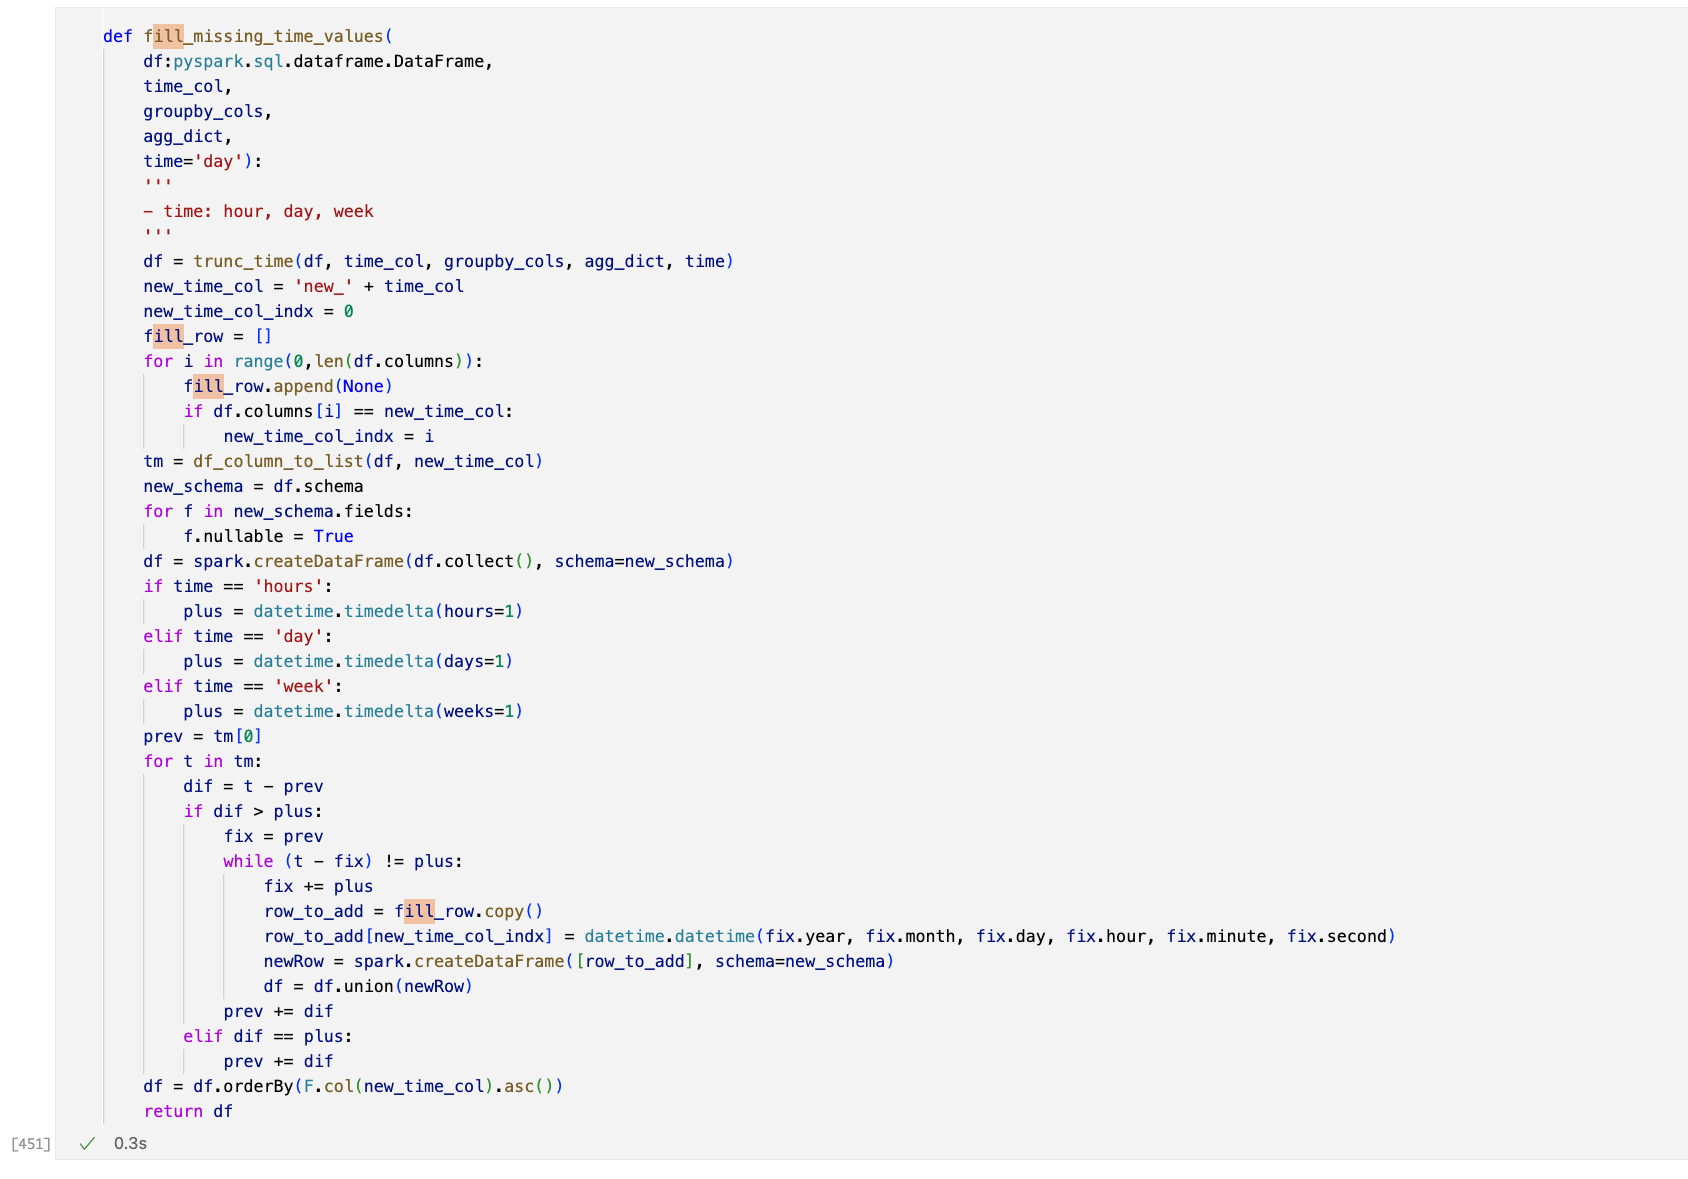
\includegraphics[scale=0.45]{3_fill_time.png}
\end{center}
\begin{center}
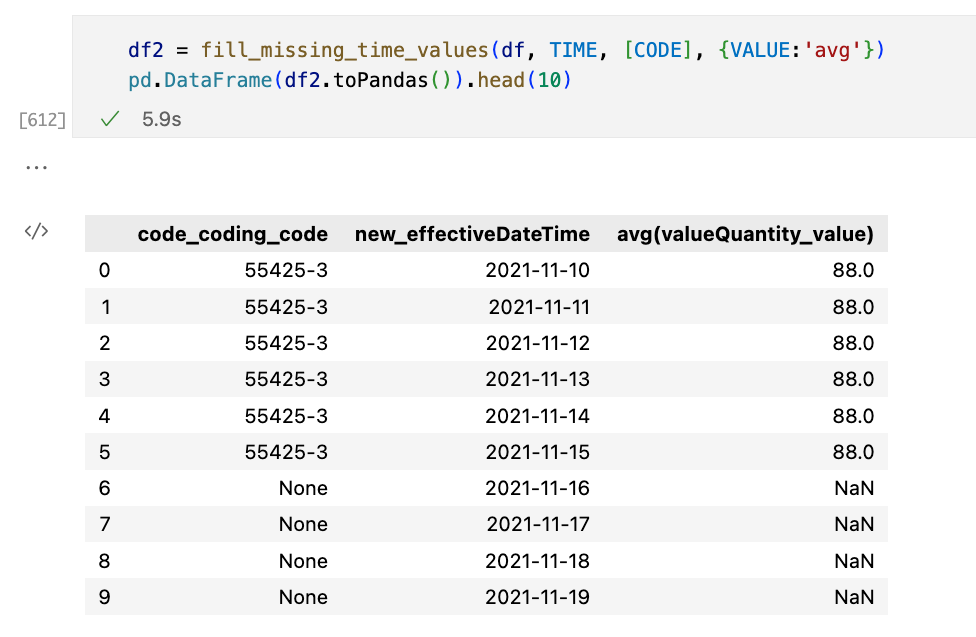
\includegraphics[scale=0.45]{3_fill_time_df.png}
\end{center}

Il dataset ottenuto risolve il problema di timestamp mancanti aggiungendo inoltre valori nulli per tutti gli altri attributi. Se ora creiamo il grafico a matrice dei dati mancanti, otteniamo spazi vuoti in corrispondenza dei timestamp aggiunti dalle precedenti funzioni.

\begin{center}
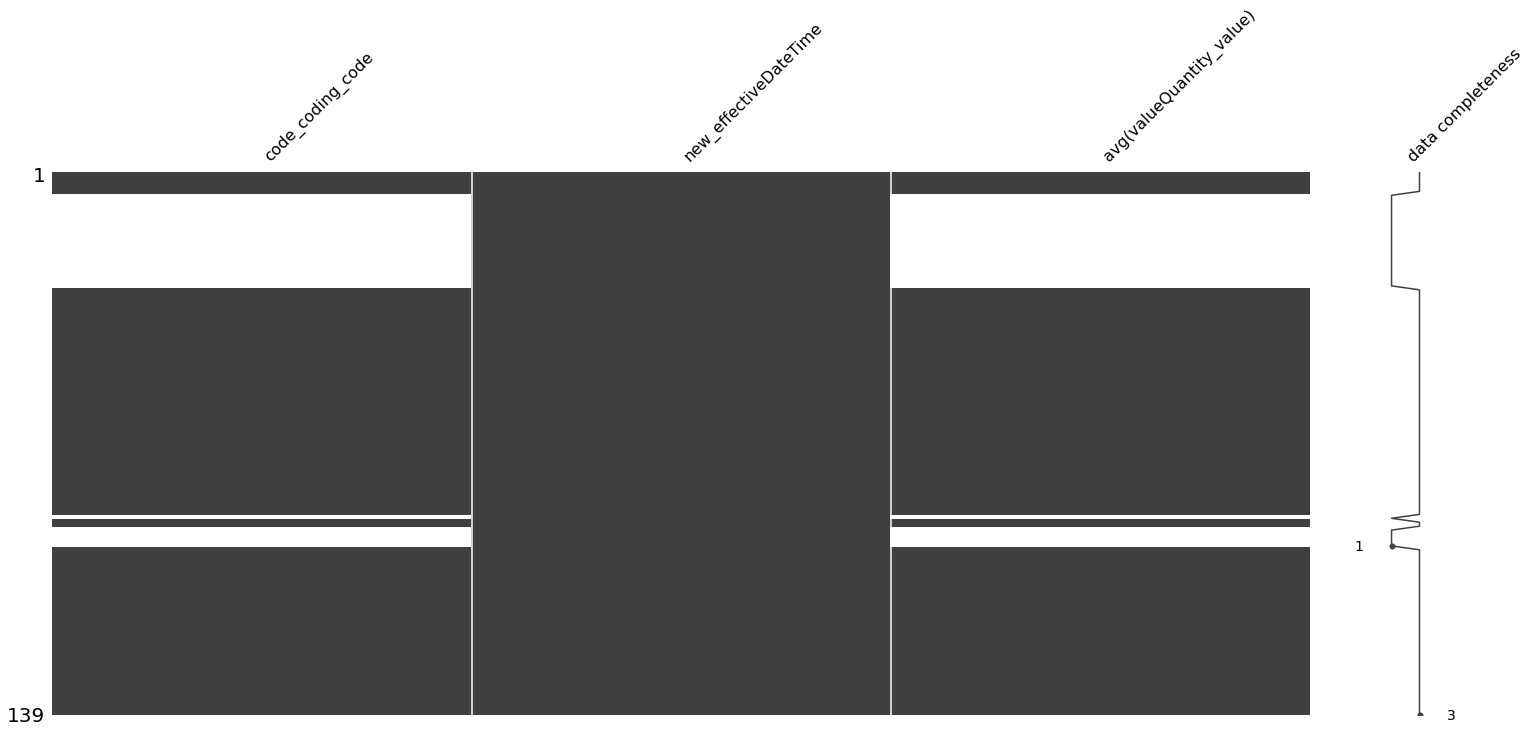
\includegraphics[scale=0.2]{2_msn_df2.png}
\end{center}

\subsection{Simple Imputer}

Per visualizzare il battito cardiaco giorno per giorno o settimana per settimana è sicuramente opportuno usare un semplice grafico come quello a linea. Lo costruiamo tramite Echarts che permette di aggiungere altri indicatori come \emph{MarkLine} e \emph{MarkPoint} che possono essere usati per segnare dati sul grafico come massimo minimo e media.

\begin{center}
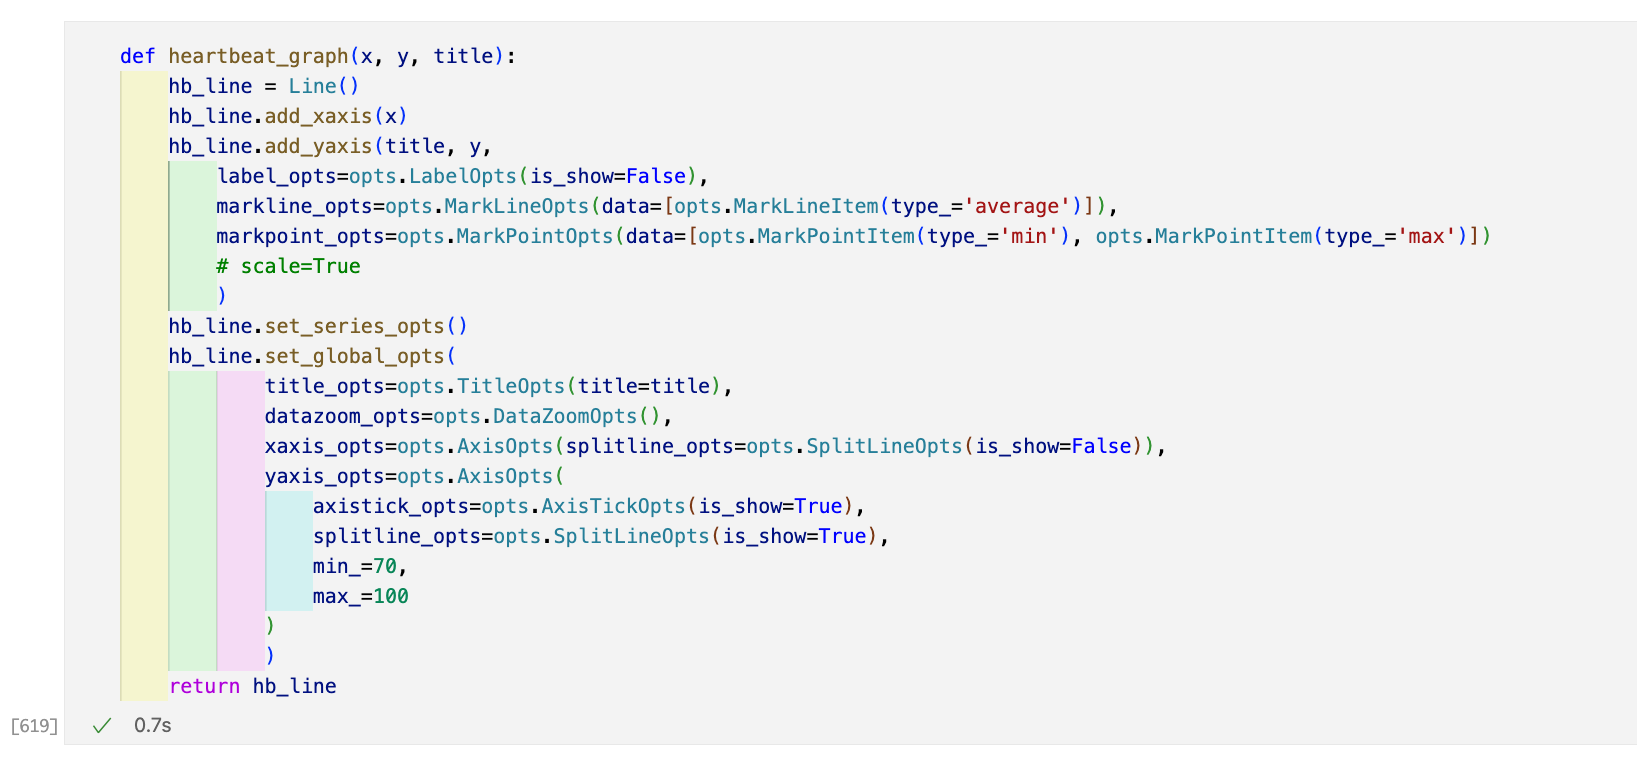
\includegraphics[scale=0.45]{4_graph.png}
\end{center}
\begin{center}
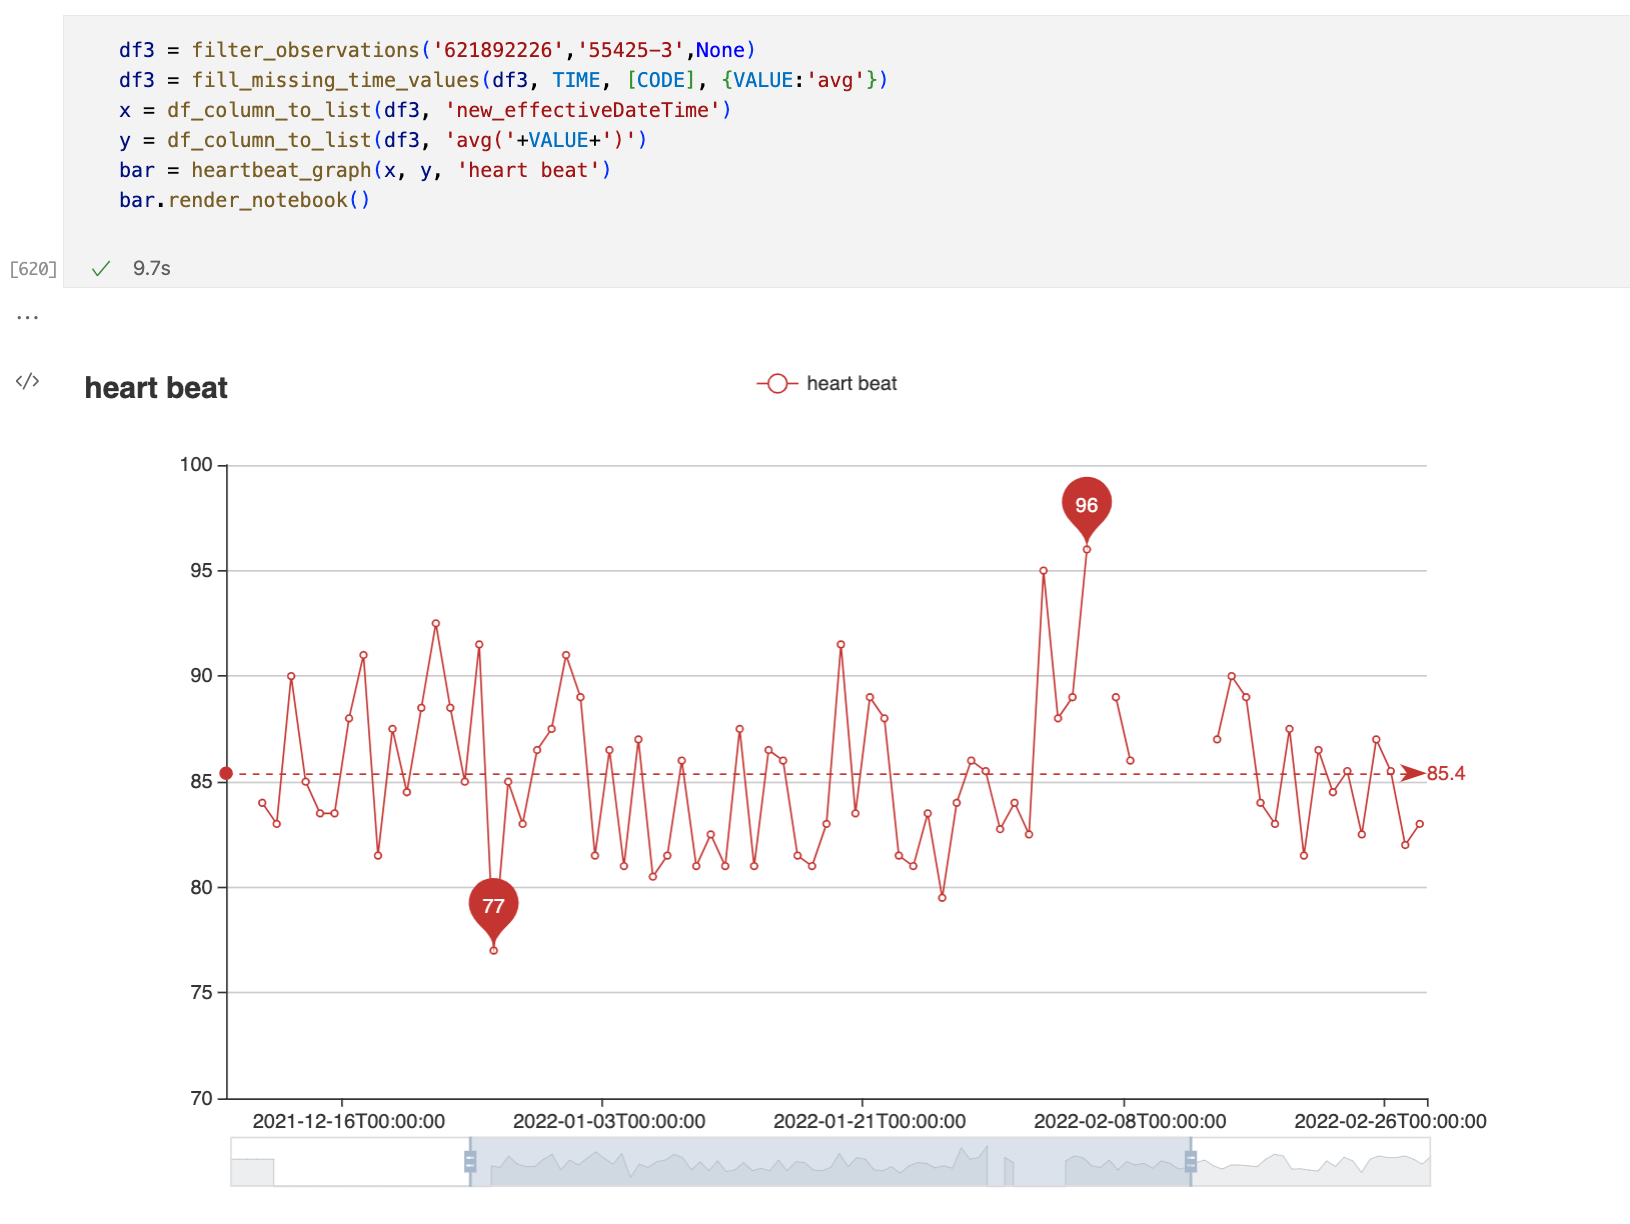
\includegraphics[scale=0.45]{4_hb.png}
\end{center}

Dal grafico ottenuto si possono facilmente vedere buchi legati alla mancanza dei dati. Ultimo passo è riempire i dati mancanti per i timestamp aggiunti in precedenza. Ci sono diverse tecniche di imputazione. Le più semplici sono sicuramente con il riempimento tramite costante, media, mediana. 

\begin{center}
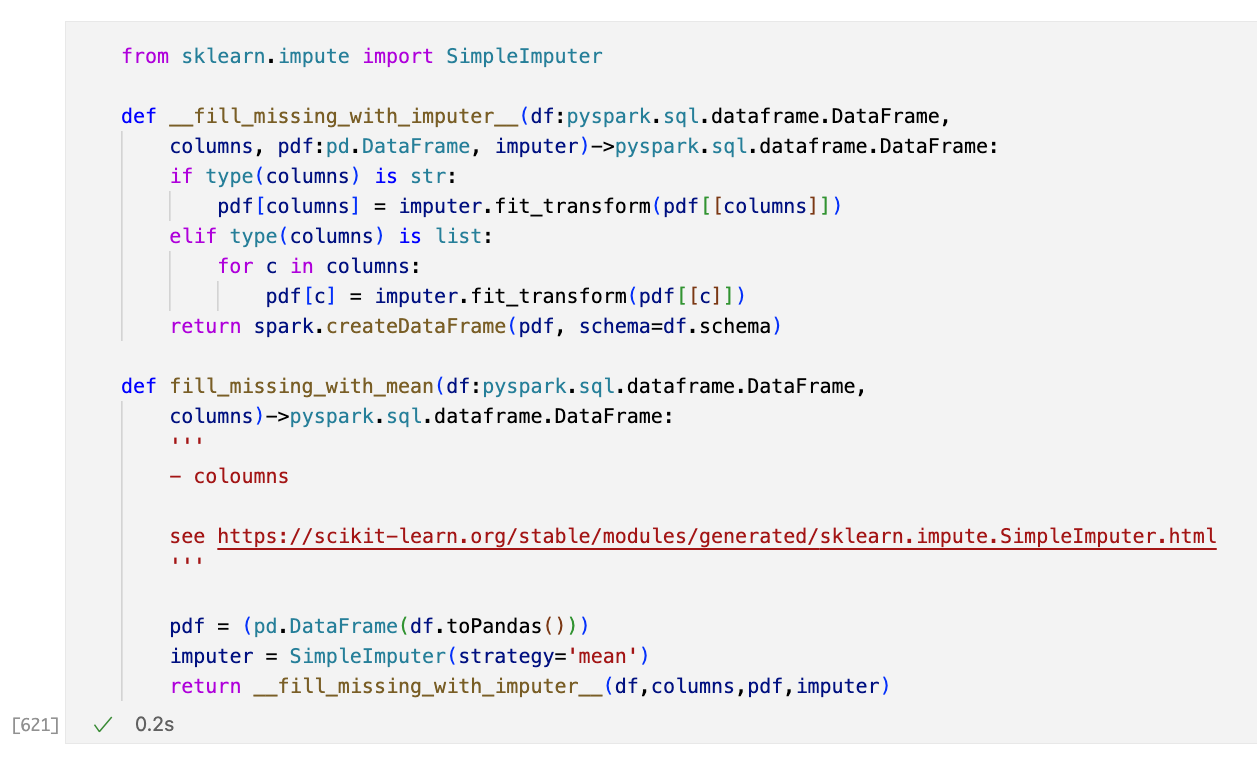
\includegraphics[scale=0.45]{4_sklearn.png}
\end{center}

Abbiamo usato una libreria come quella di \emph{Sklearn} che contiene funzionalità come quella di \emph{SimpleImputer} per creare una semplice funzione che riempie i dati mancanti di una qualsiasi colonna di un DataFrame PySpark.

\begin{center}
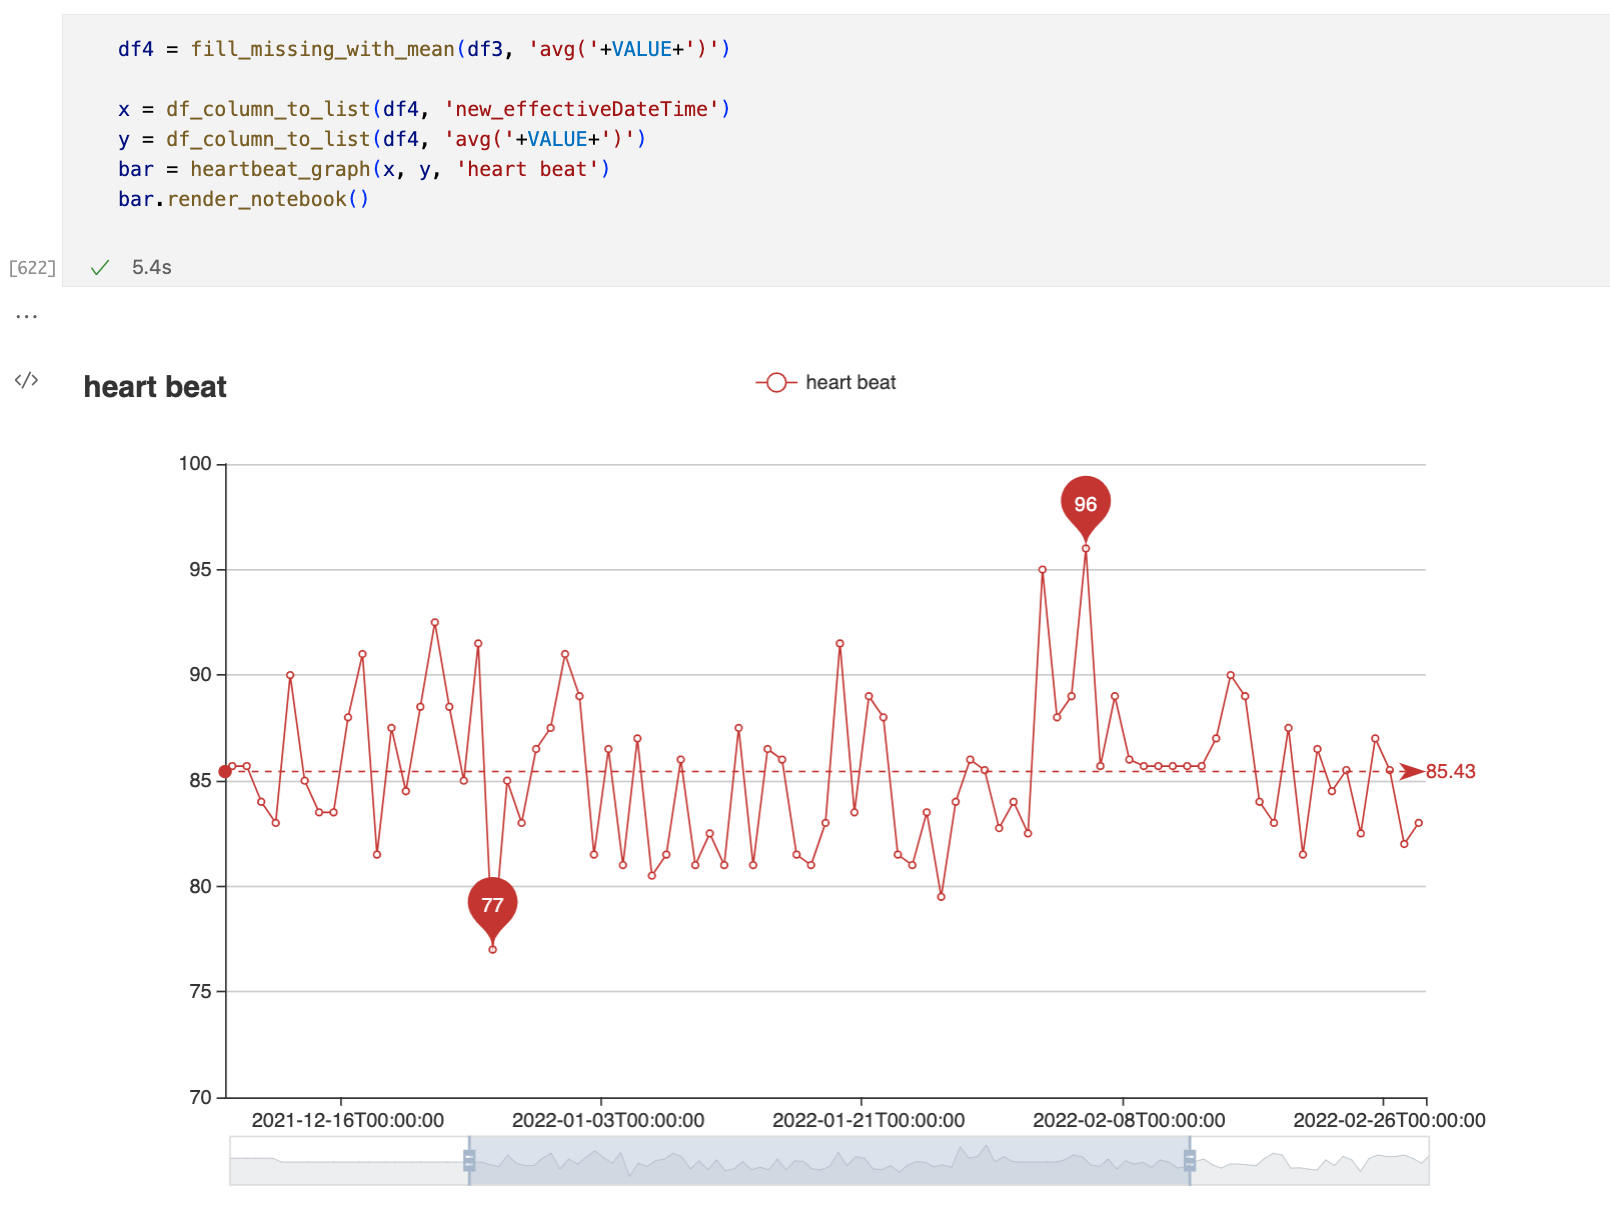
\includegraphics[scale=0.45]{4_hb_mean.png}
\end{center}

Il grafico risultante non contiene più valori mancanti e quindi spazi vuoti. Vi sono anche tecniche gradualmente più complesse per ricavare i dati mancanti partendo da quelli presenti, come Linear Regression, KNN, MICE, e altre.

\subsection{Extensions}

Grazie alle funzioni precedentemente descritte possiamo visualizzare l'andamento del battito cardiaco settimana per settimana e creare una gif animata della sua progressione nel tempo. Utilizzando una libreria come \emph{imageio} raggruppiamo tutti i grafici dell'oscillazione per ogni settimana ottenendo una gif che mostra la progressione del battito cardiaco per un totale di 20 settimane.  

\begin{center}
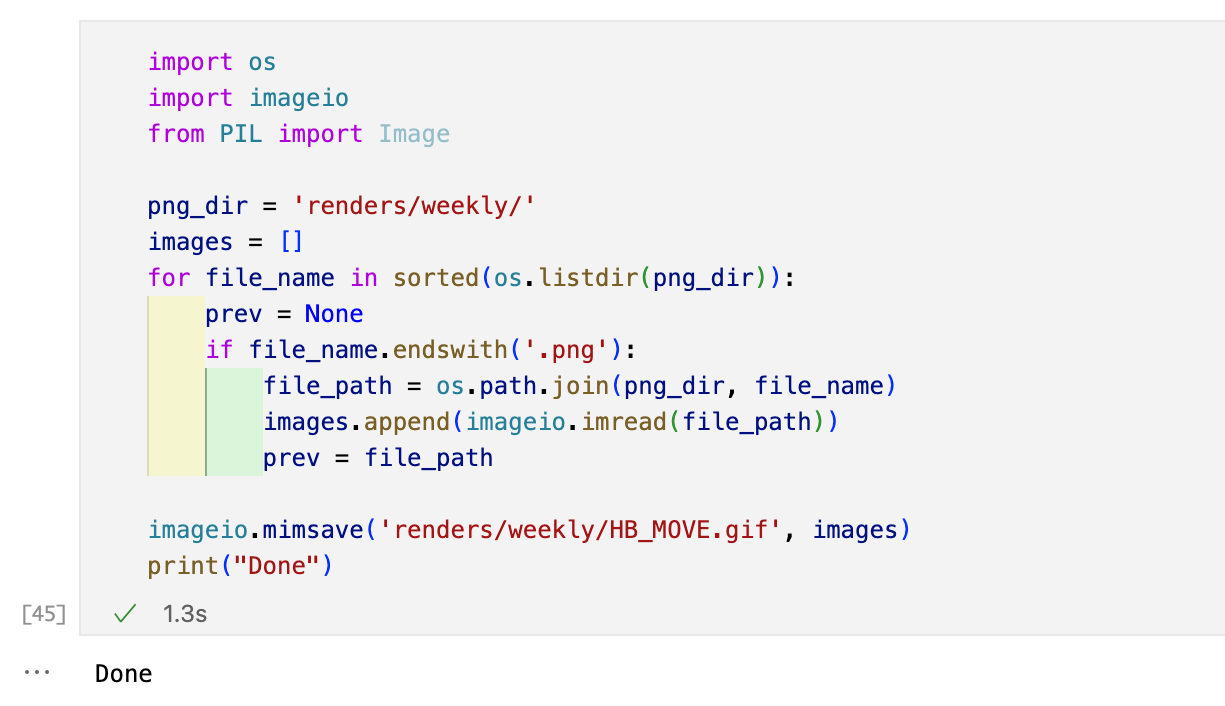
\includegraphics[scale=0.45]{5_gif.png}
\end{center}

\begin{center}
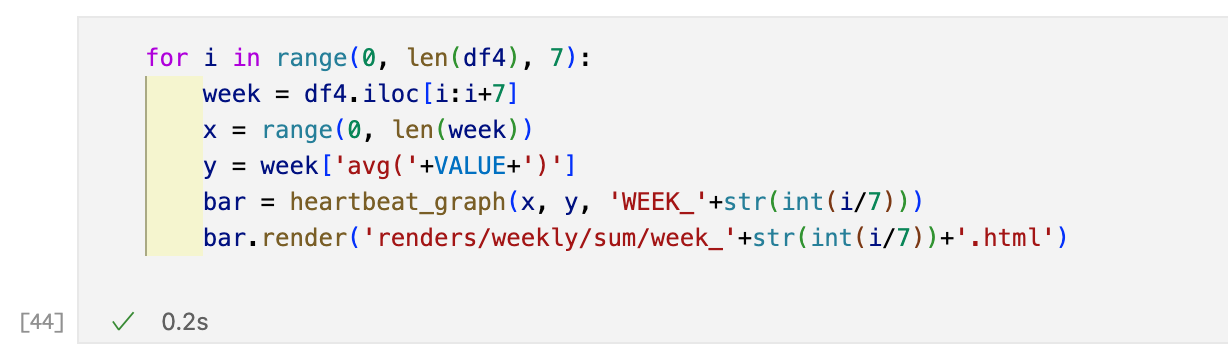
\includegraphics[scale=0.45]{5_mk_gif_1.png}
\end{center}

\begin{center}
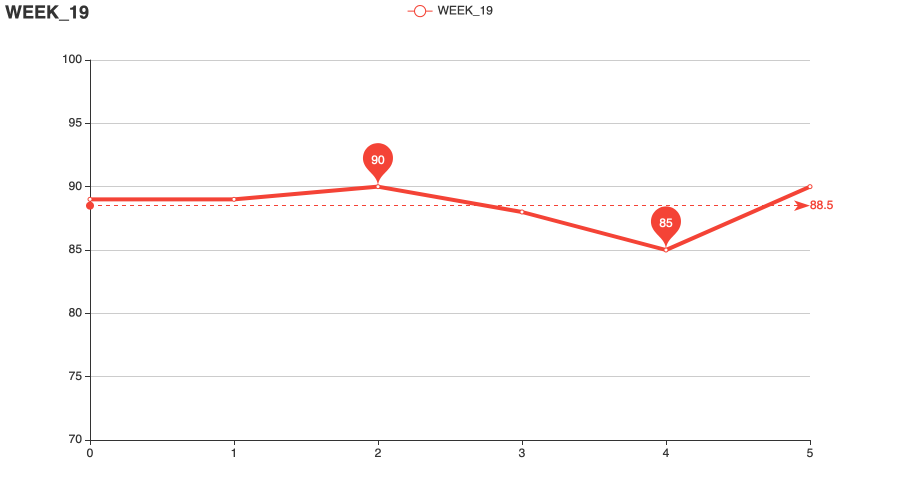
\includegraphics[scale=0.4]{5_hb.png}
\end{center}

Un'altra estensione per questa visualizzazione animata può essere quella di salvare e visualizzare anche le settimane precedenti in modo tale da confrontarle mano a mano che il tempo passa. Il grafico ottenuto ad ogni frame conterrà in grigio sbiadito le settimane precedenti mentre in rilievo la settimana corrente.

\begin{center}
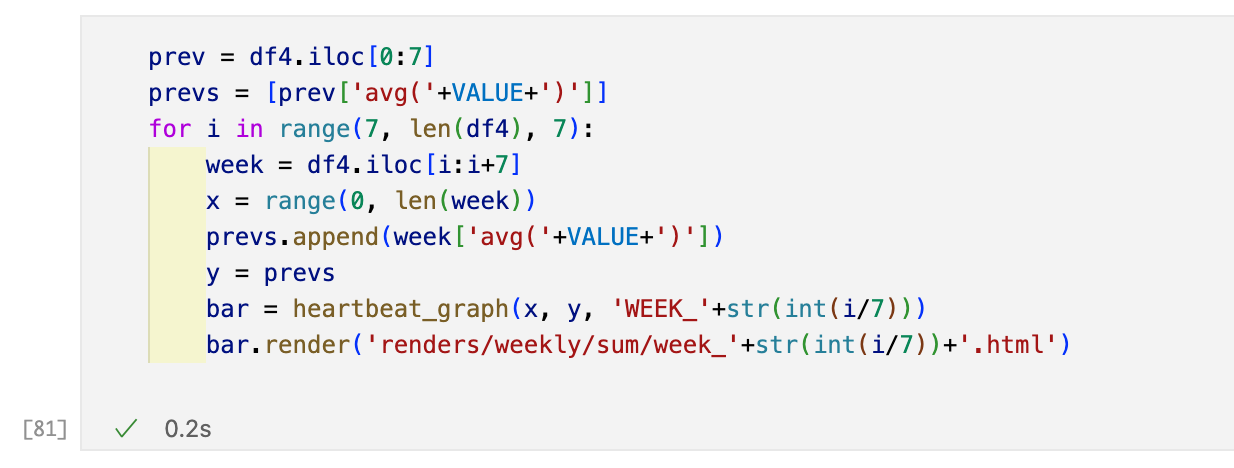
\includegraphics[scale=0.45]{5_mk_gif_2.png}
\end{center}

\begin{center}
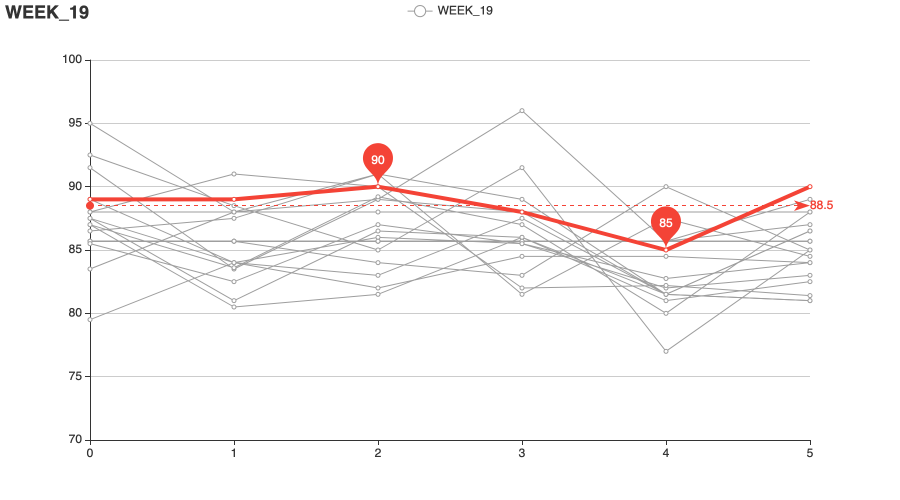
\includegraphics[scale=0.4]{5_hb_sum.png}
\end{center}

\end{document}  